%!TEX root = ../AliStrangeJets.tex

\section{Results and discussion}%
\label{sec:Results}

\subsection{Particles $\pT$-differential density}
\label{subsec:ParPtDensity}

For the strange hadrons discussed in this paper, the ratios of yields for particles and anti-particles are around one within the uncertainties, as expected at these collision energies in the mid-rapidity region.
Therefore, all the $\pT$-differential density shown in the following are reported after summing particles and anti-particles.
The different selections shown in the following have been introduced in section~\ref{sec:ParJetMatch}, inwhich also introduced the normalization method. 

Figure~\ref{fig:ppSpect} shown the $\kzero$, $\lmb + \almb$, $\X + \Ix$ and $\Om + \Mo$ $\pT$-differential density distributions in \pp collisions.


\begin{figure}[!ht]
	\begin{center}
		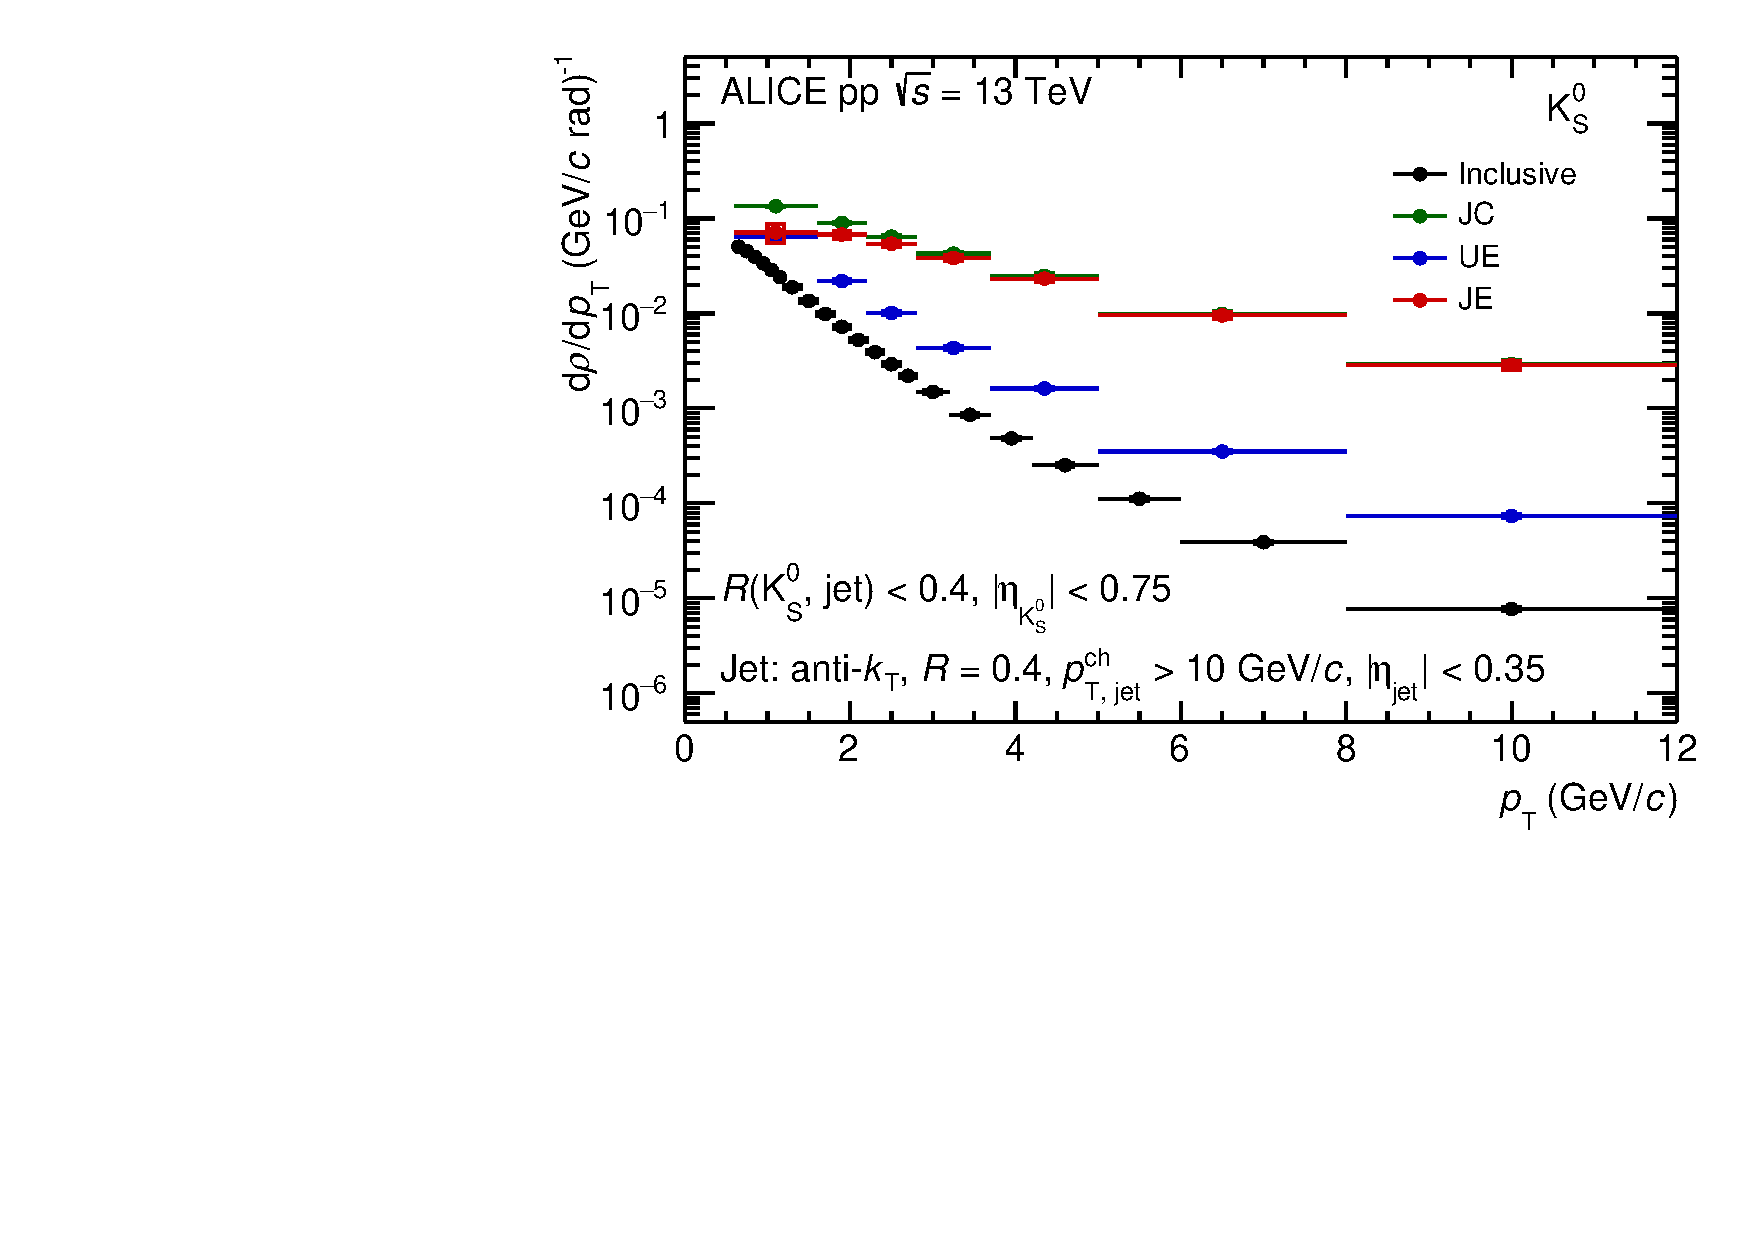
\includegraphics[width=.4\textwidth]{cf4_1}
		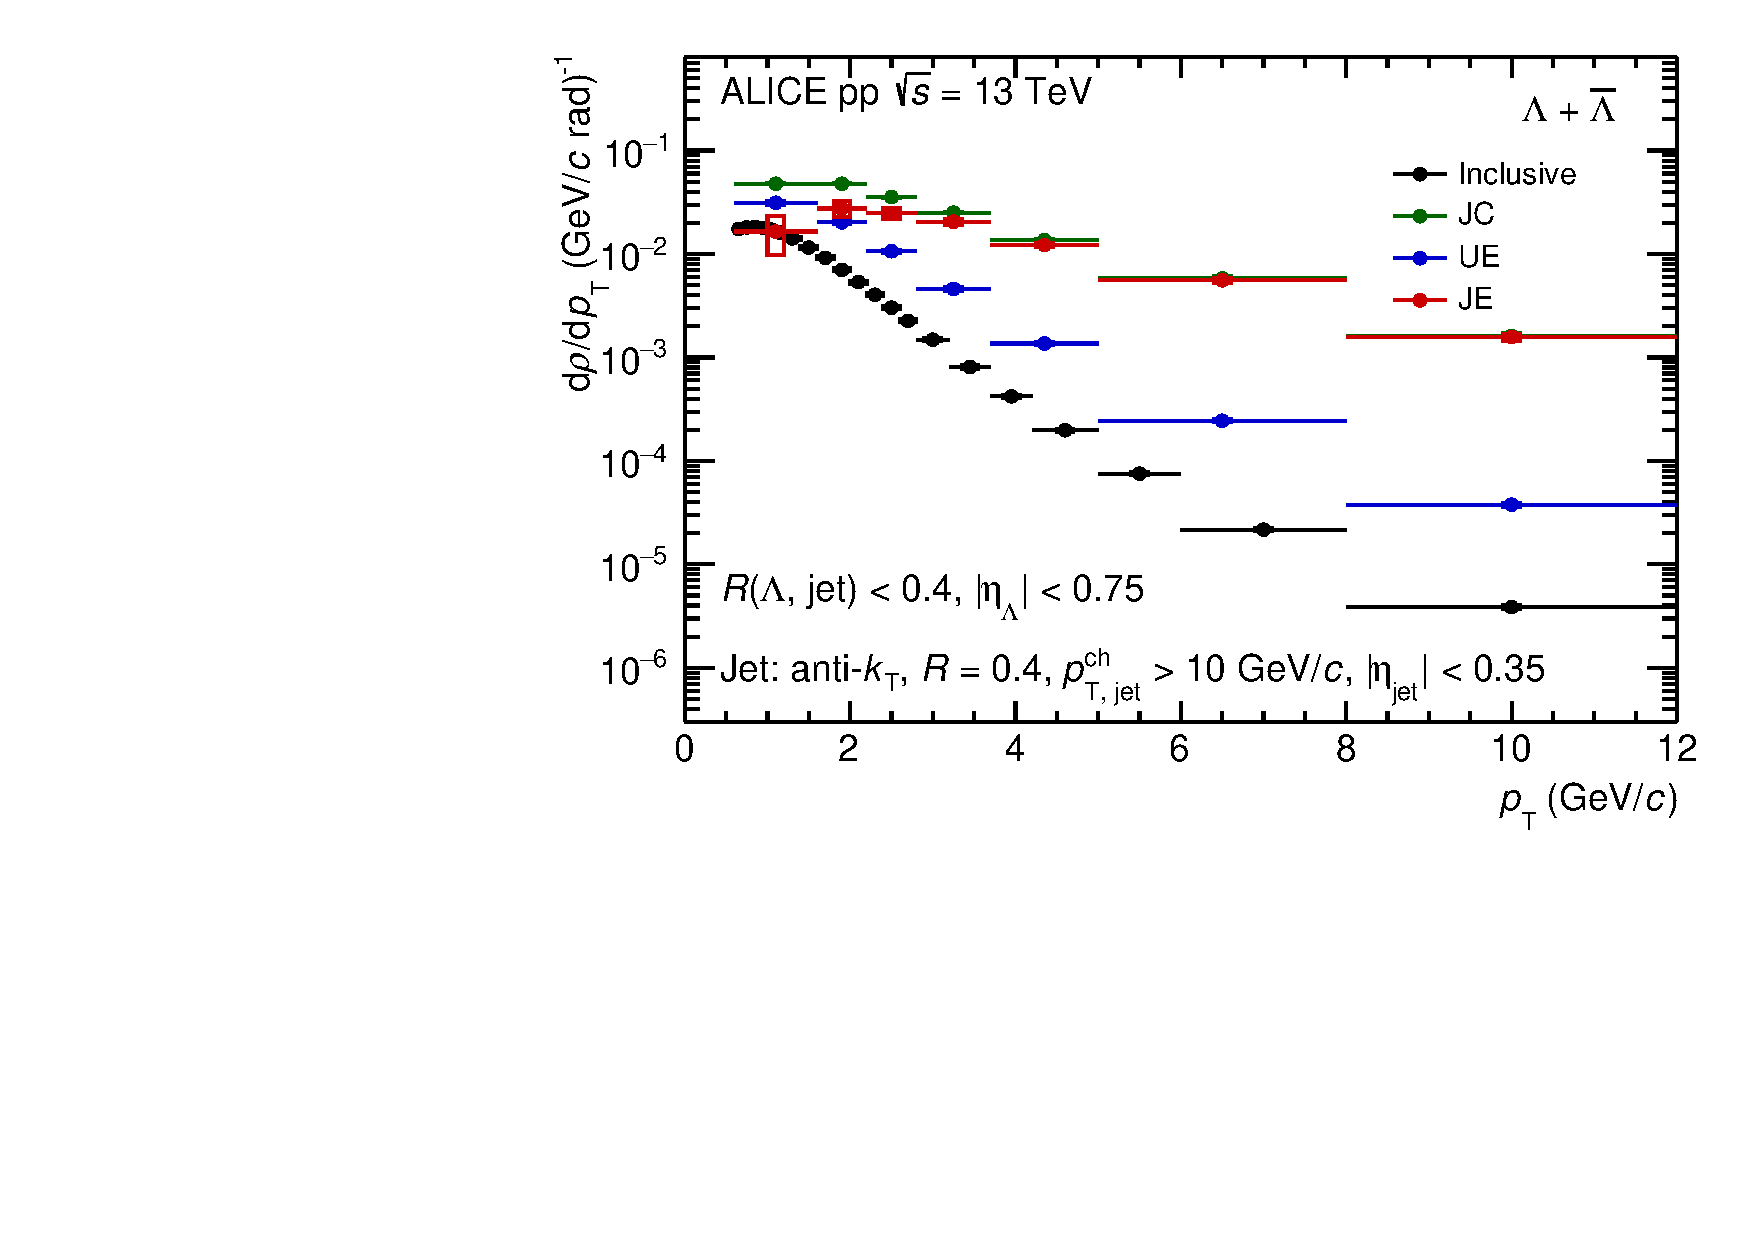
\includegraphics[width=.4\textwidth]{cf4_2}
		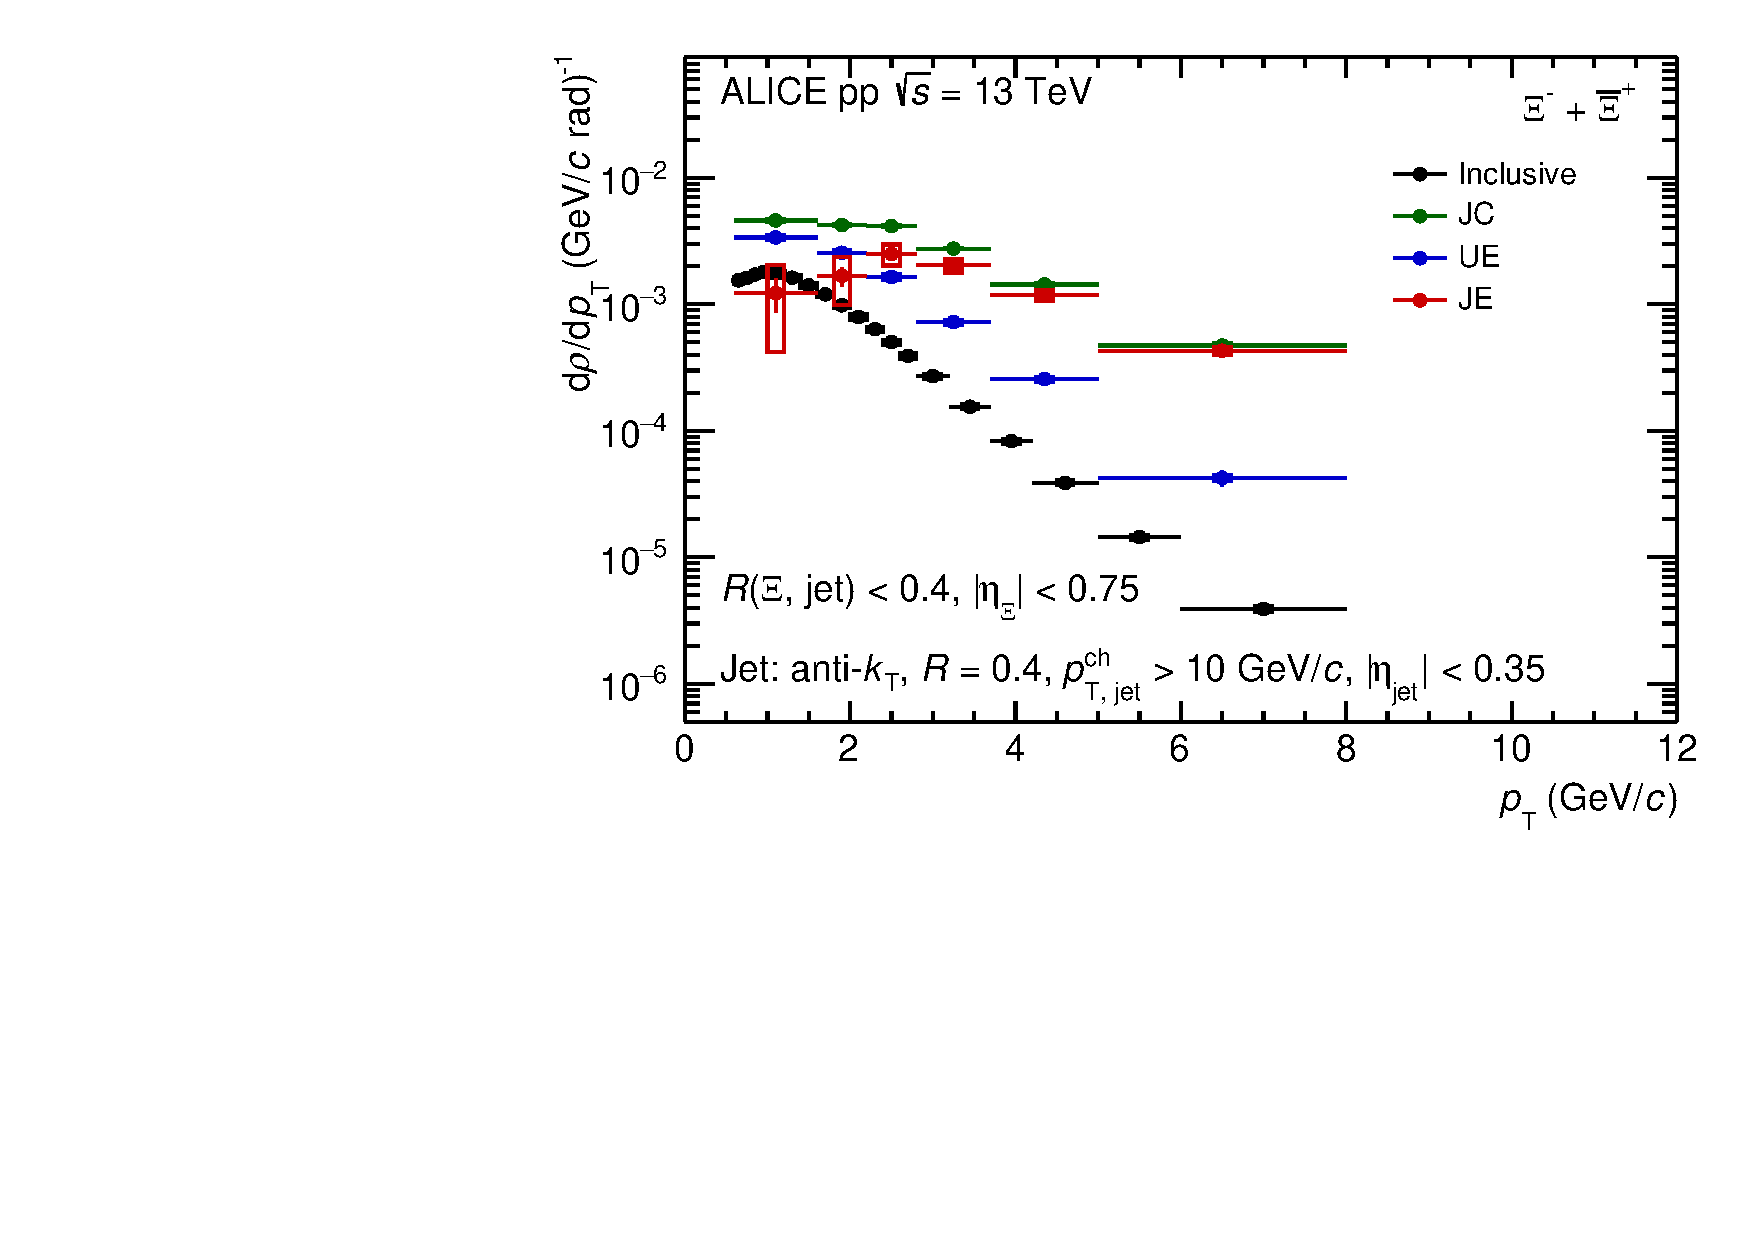
\includegraphics[width=.4\textwidth]{cf4_3}
		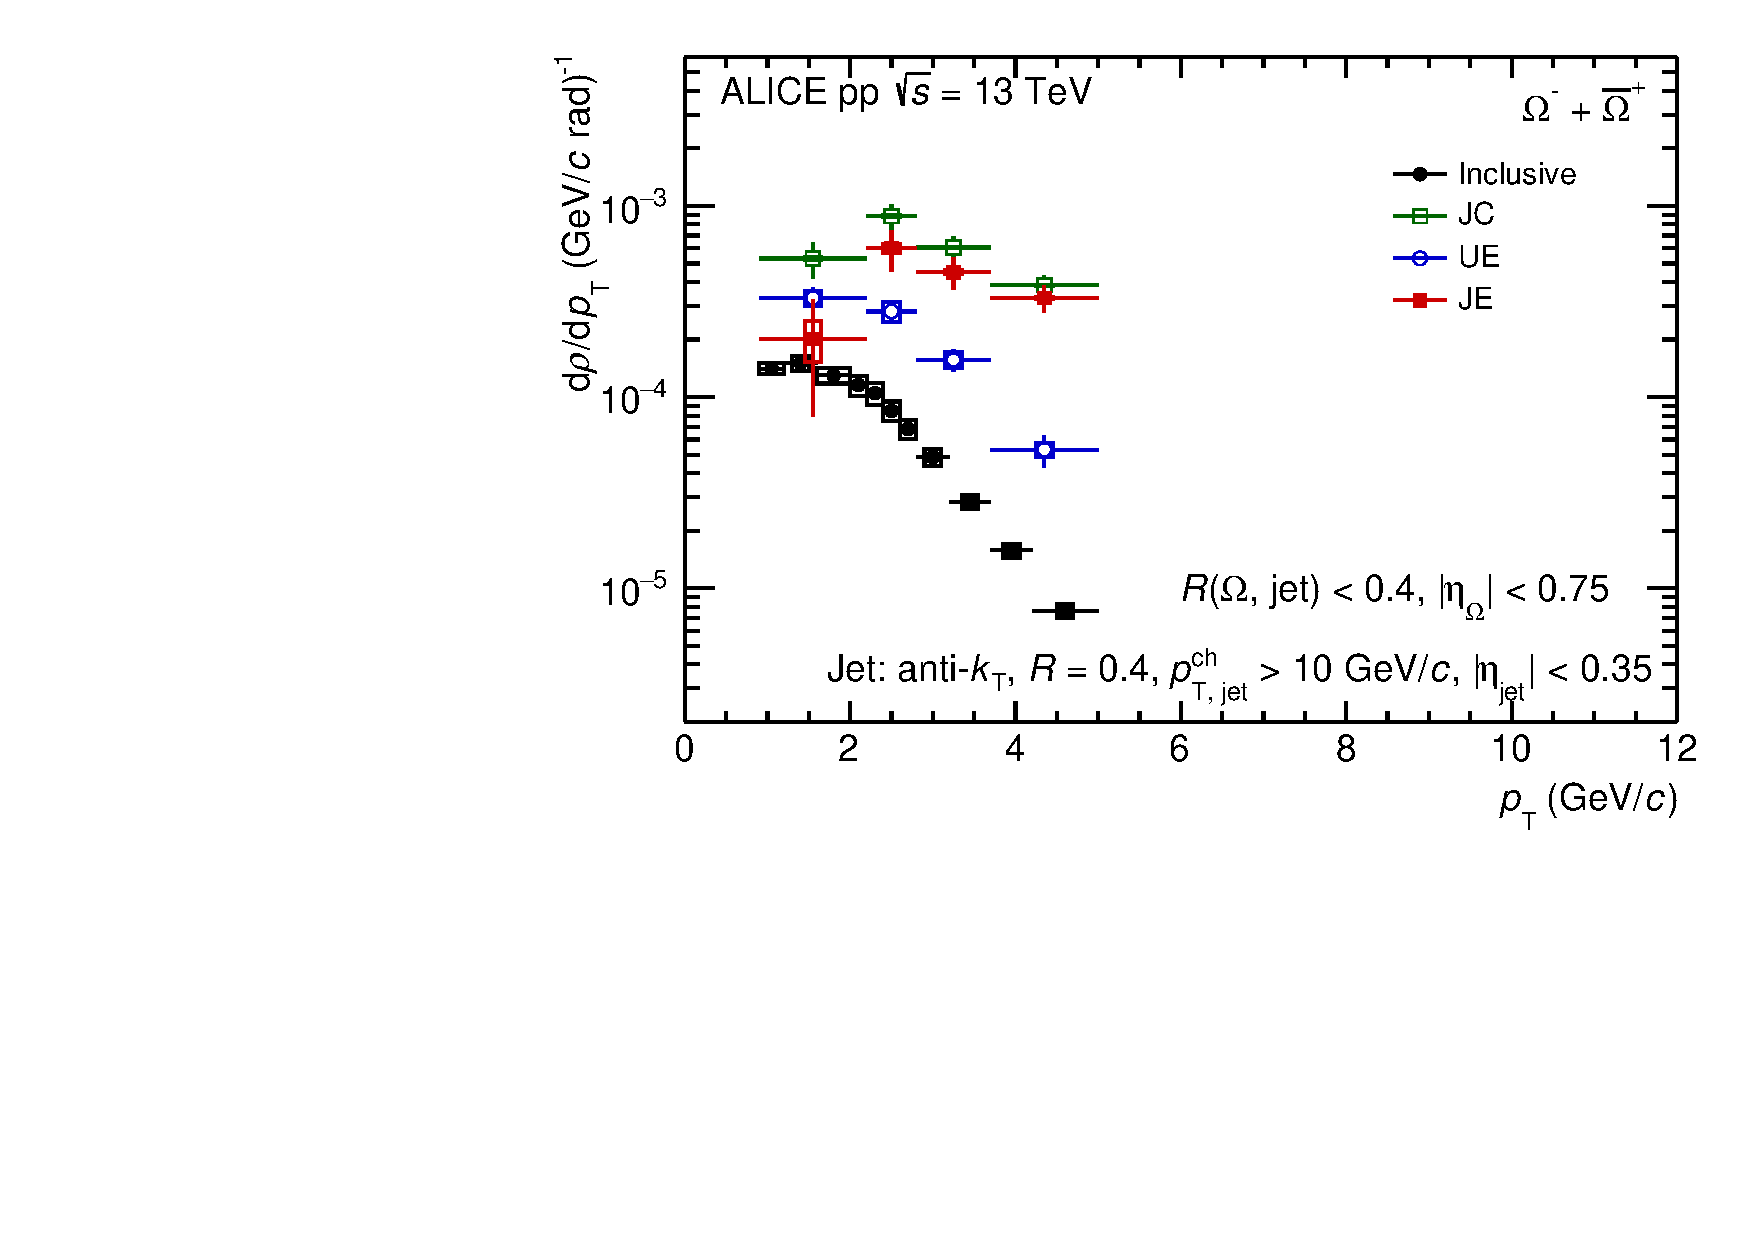
\includegraphics[width=.4\textwidth]{cf4_4}
	\end{center}
	\caption{$\pT$-differential density of strange hadrons in \pp at \thirteen.}
	\label{fig:ppSpect}
\end{figure}
\begin{figure}[!ht]
	\begin{center}
		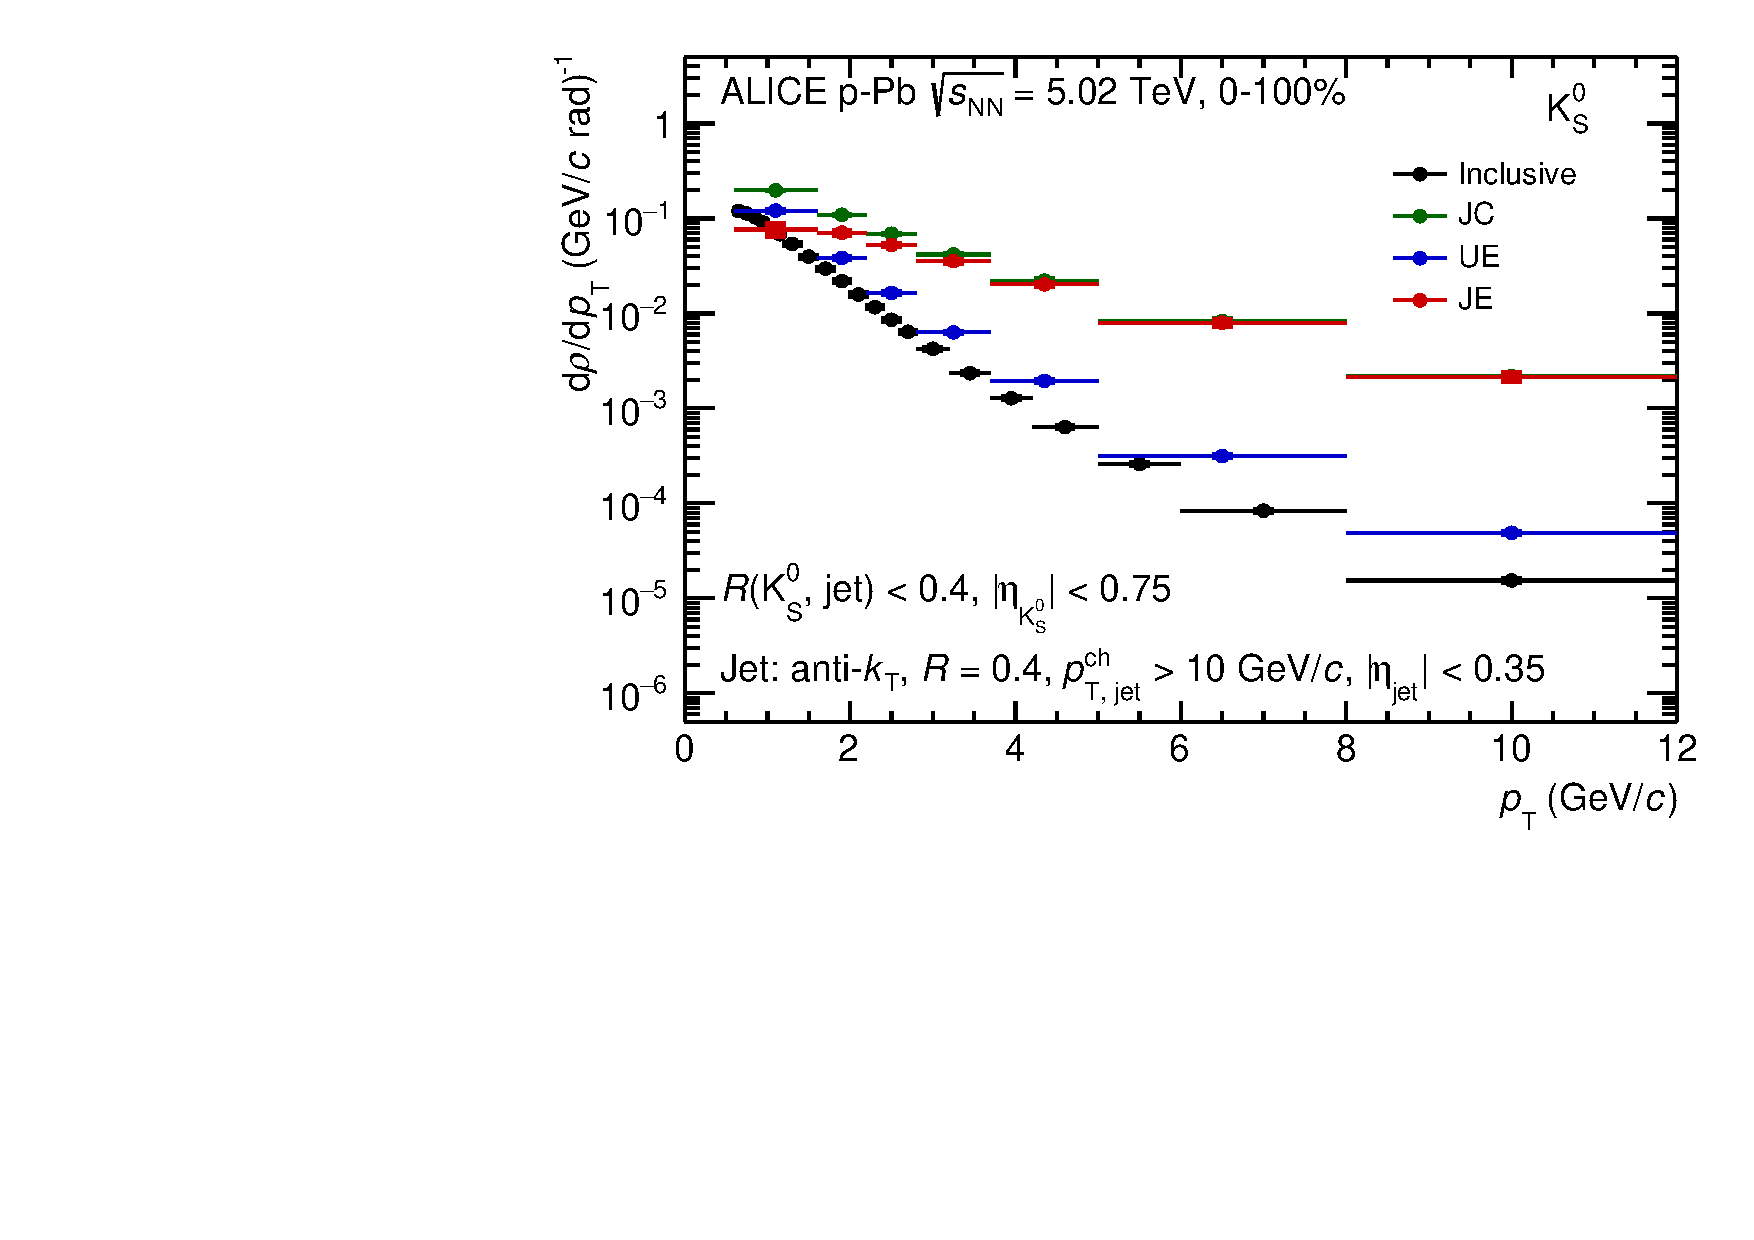
\includegraphics[width=.4\textwidth]{cf5_1}
		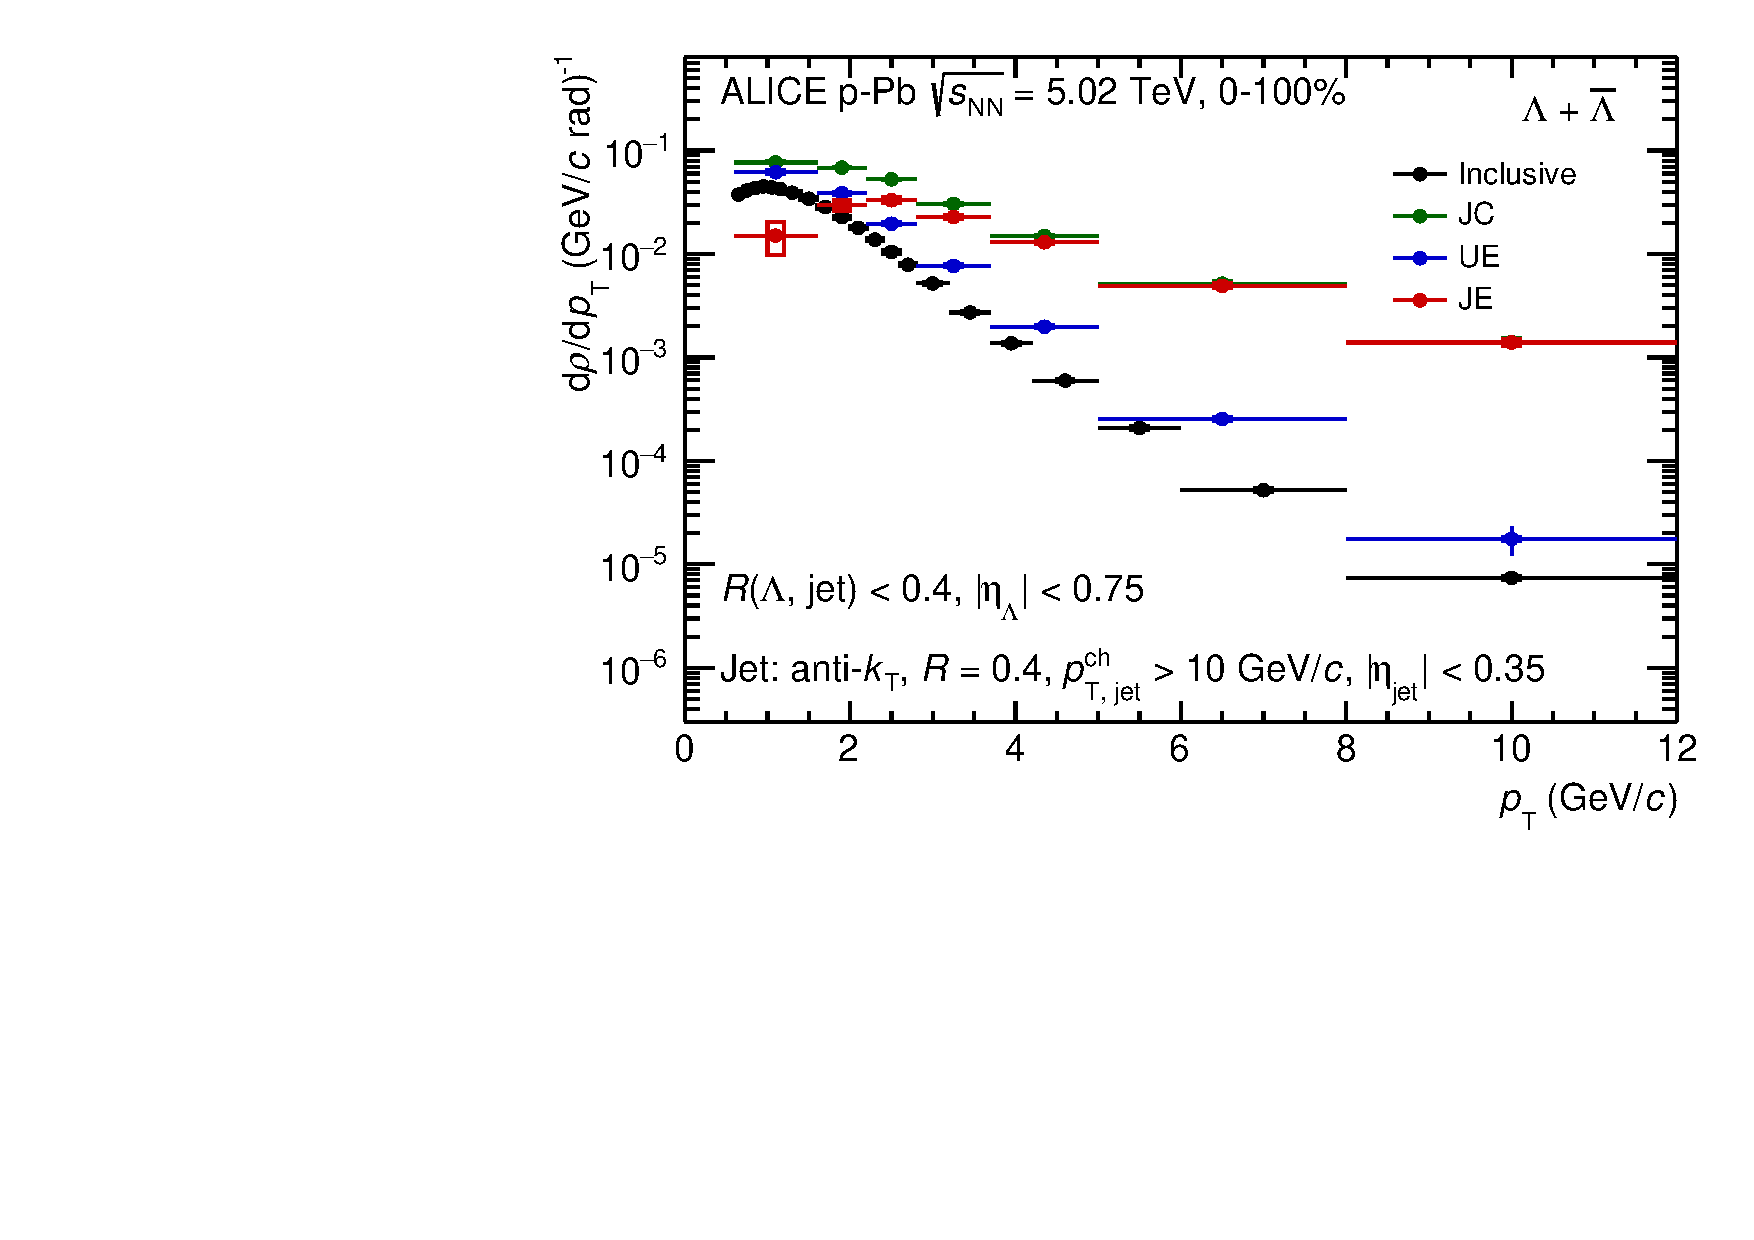
\includegraphics[width=.4\textwidth]{cf5_2}
		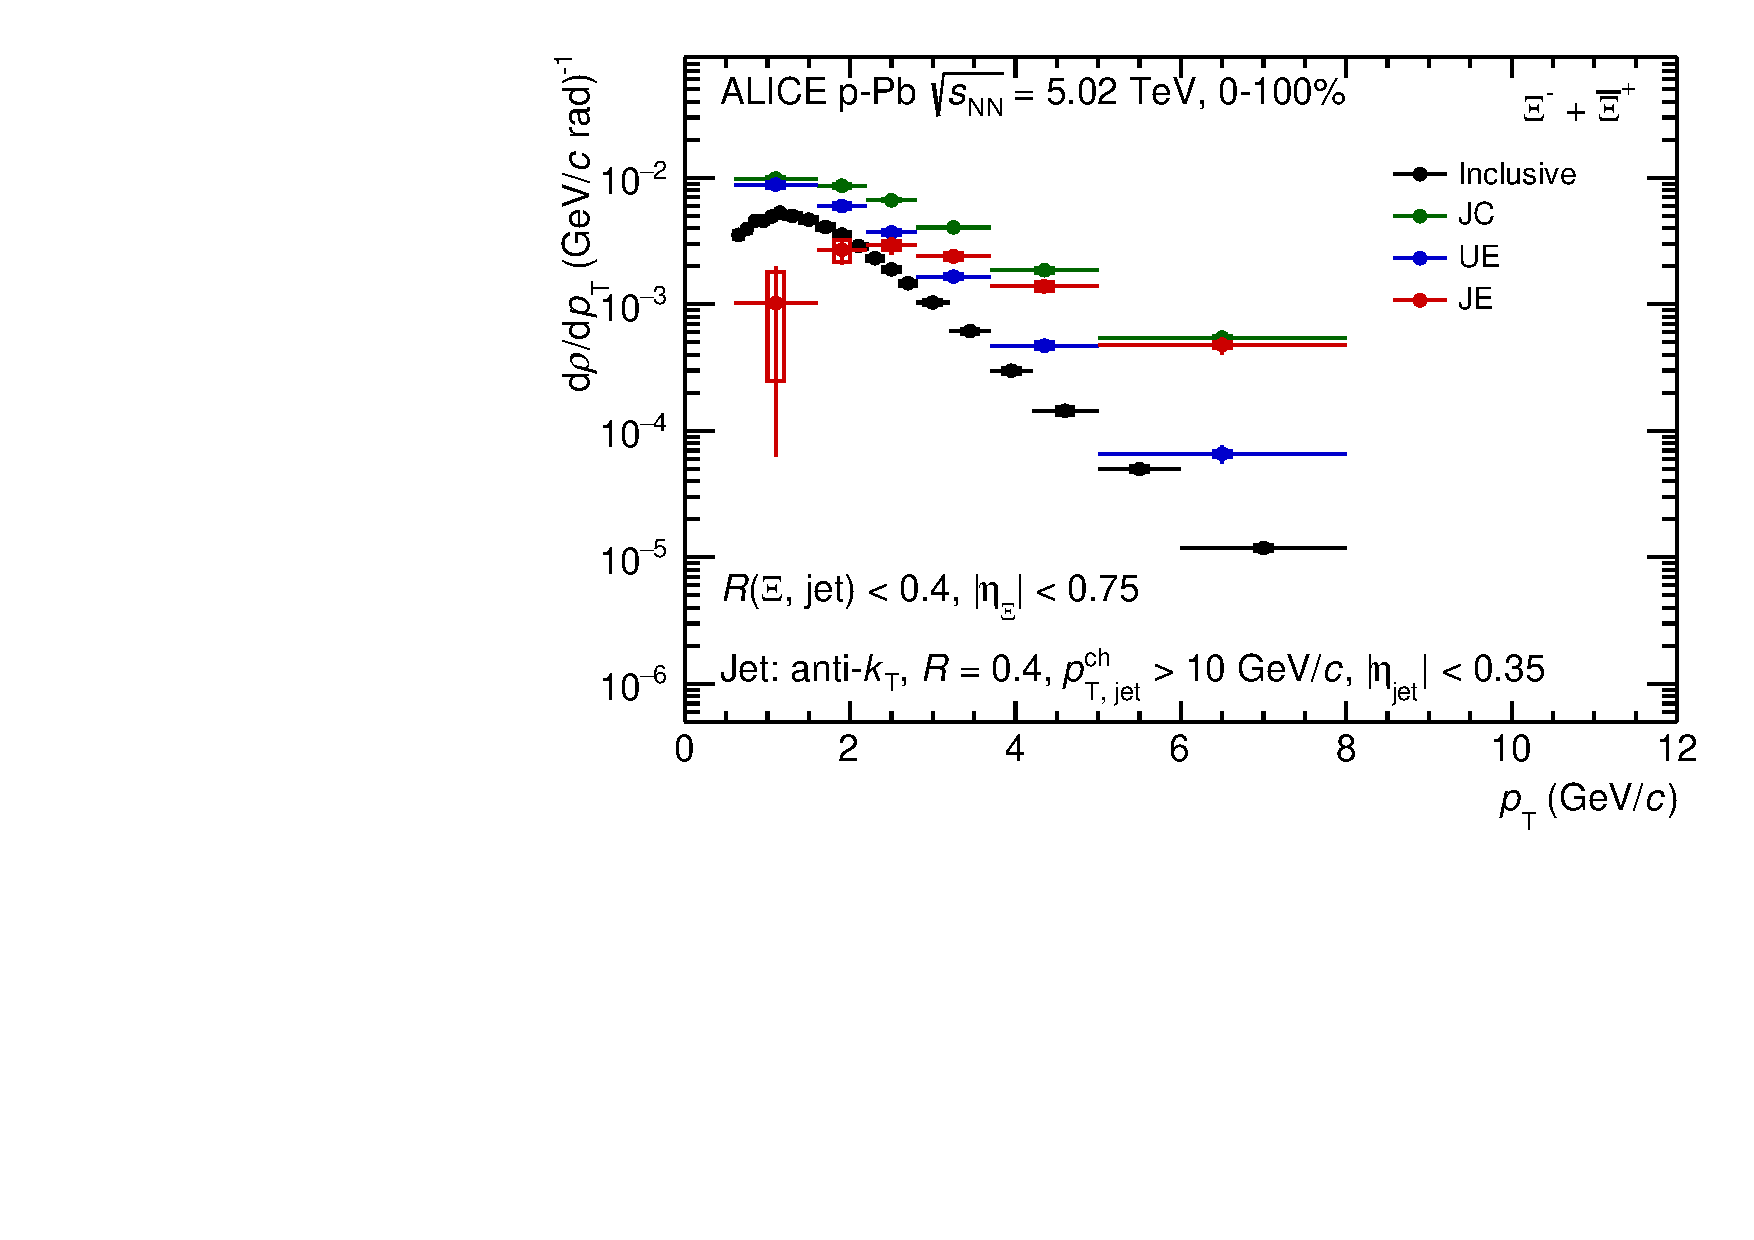
\includegraphics[width=.4\textwidth]{cf5_3}
		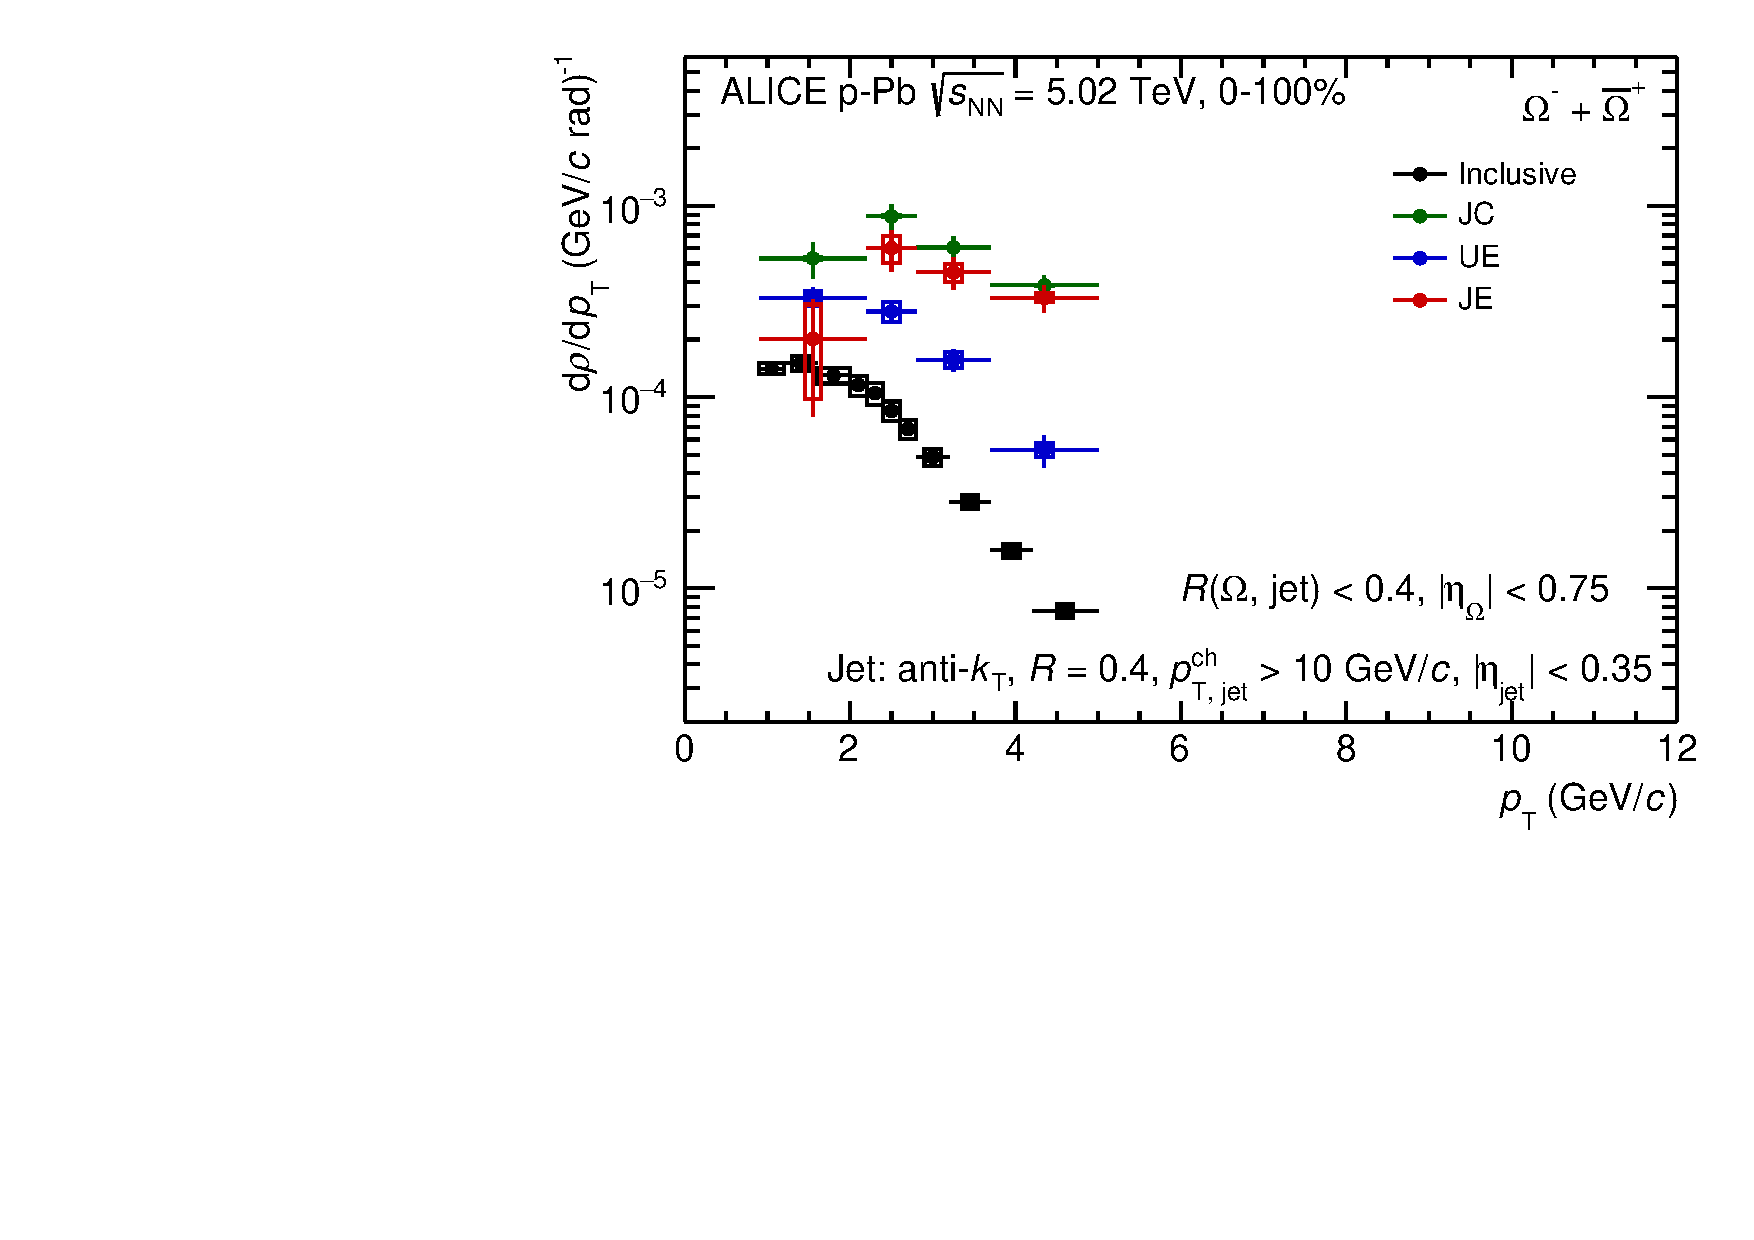
\includegraphics[width=.4\textwidth]{cf5_4}
	\end{center}
	\caption{$\pT$-differential density of strange hadrons in 0-100\% in \pPb in \fivenn.}
	\label{fig:pPbSpect}
\end{figure}
\begin{figure}[!ht]
\begin{center}
	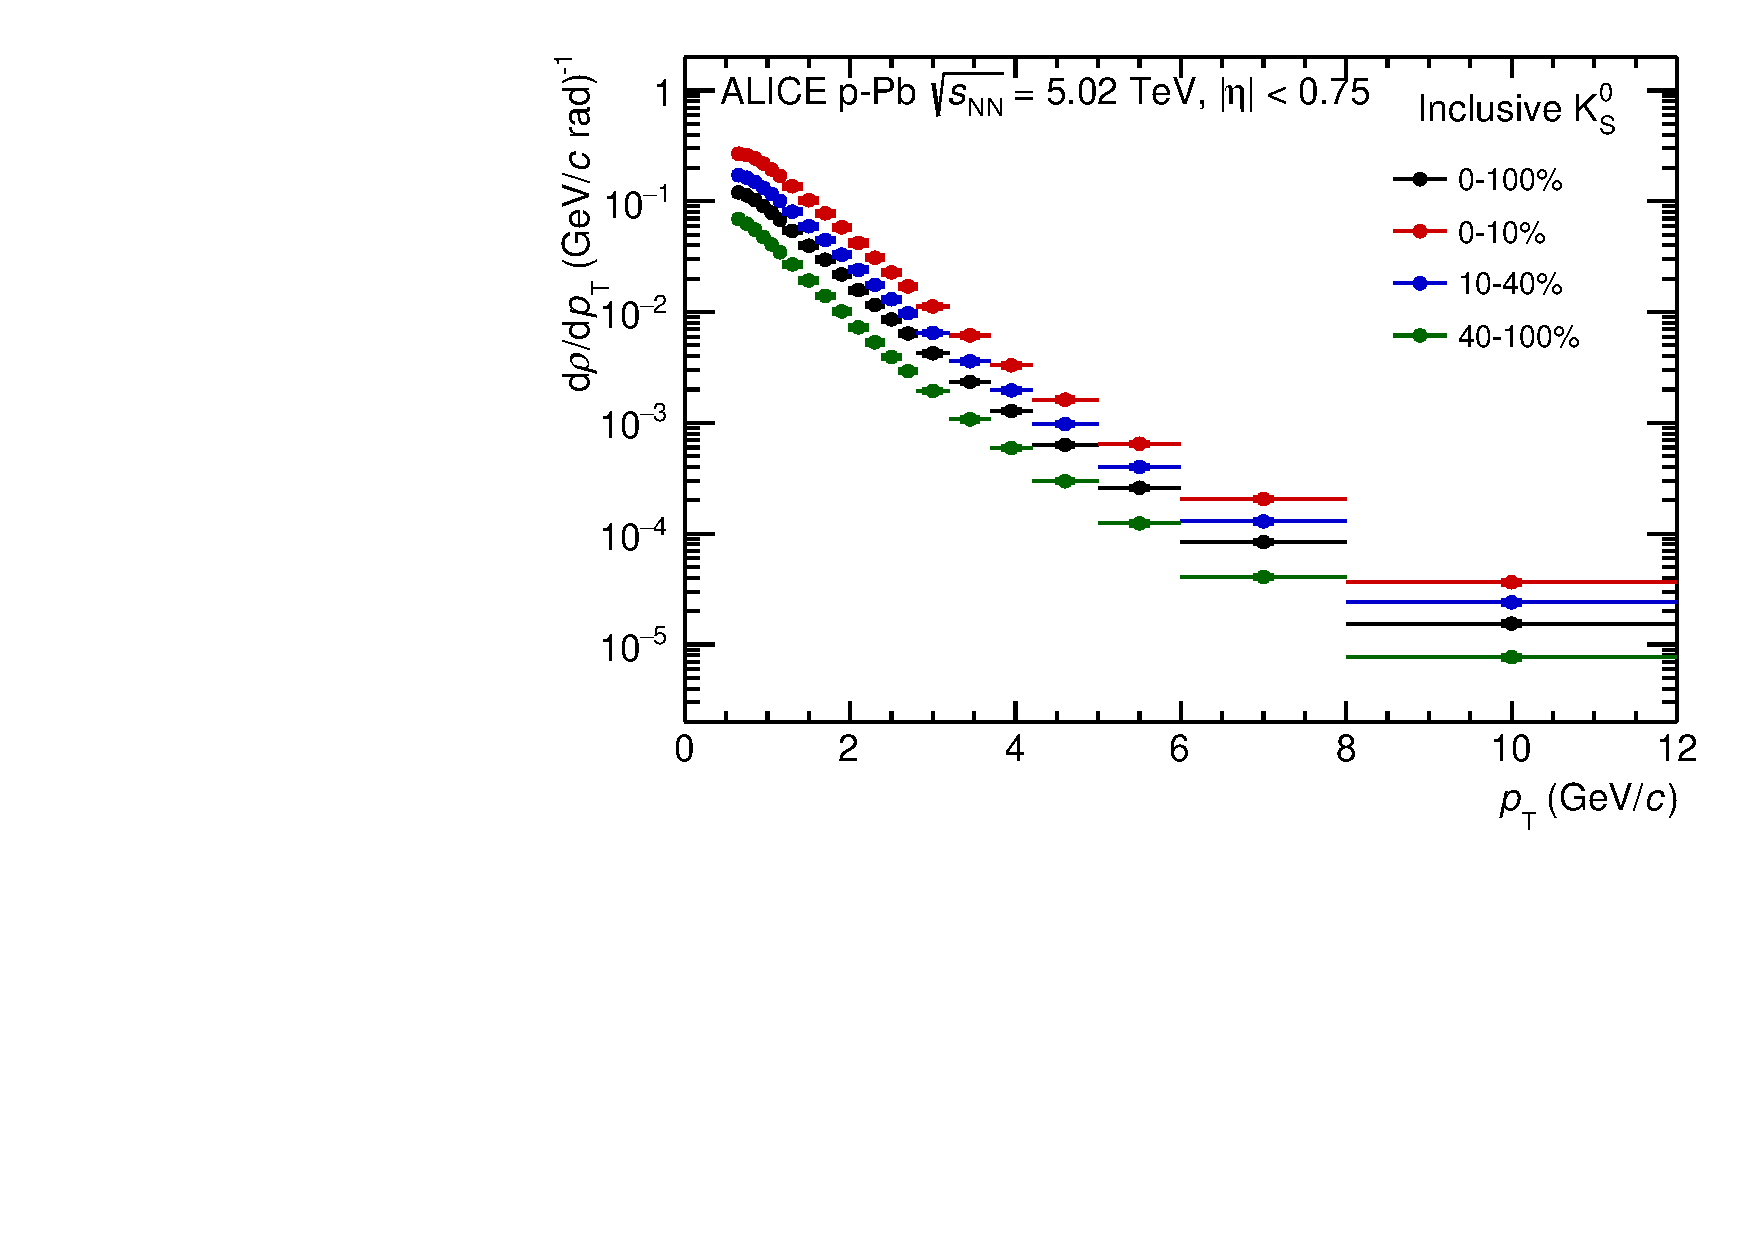
\includegraphics[width=.3\textwidth]{cf6_1}
	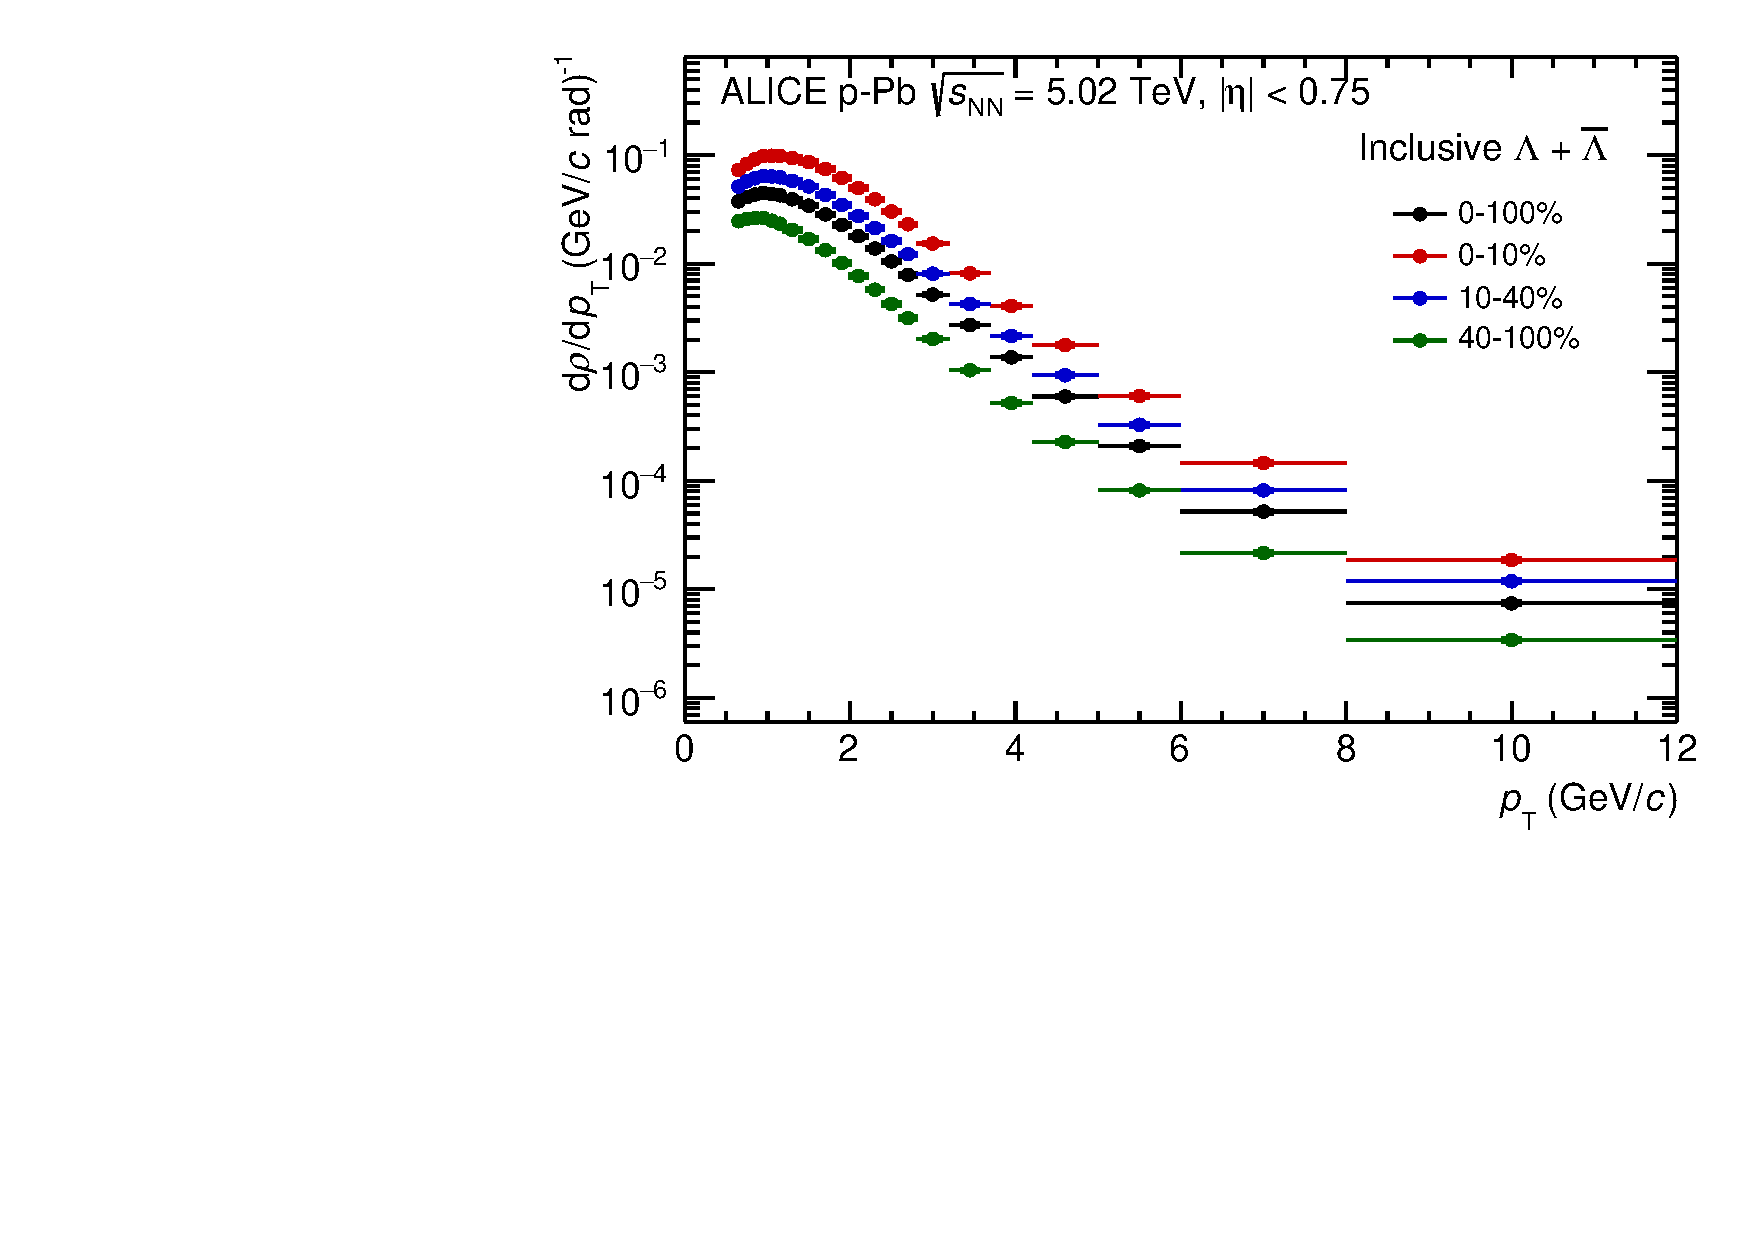
\includegraphics[width=.3\textwidth]{cf6_2}
	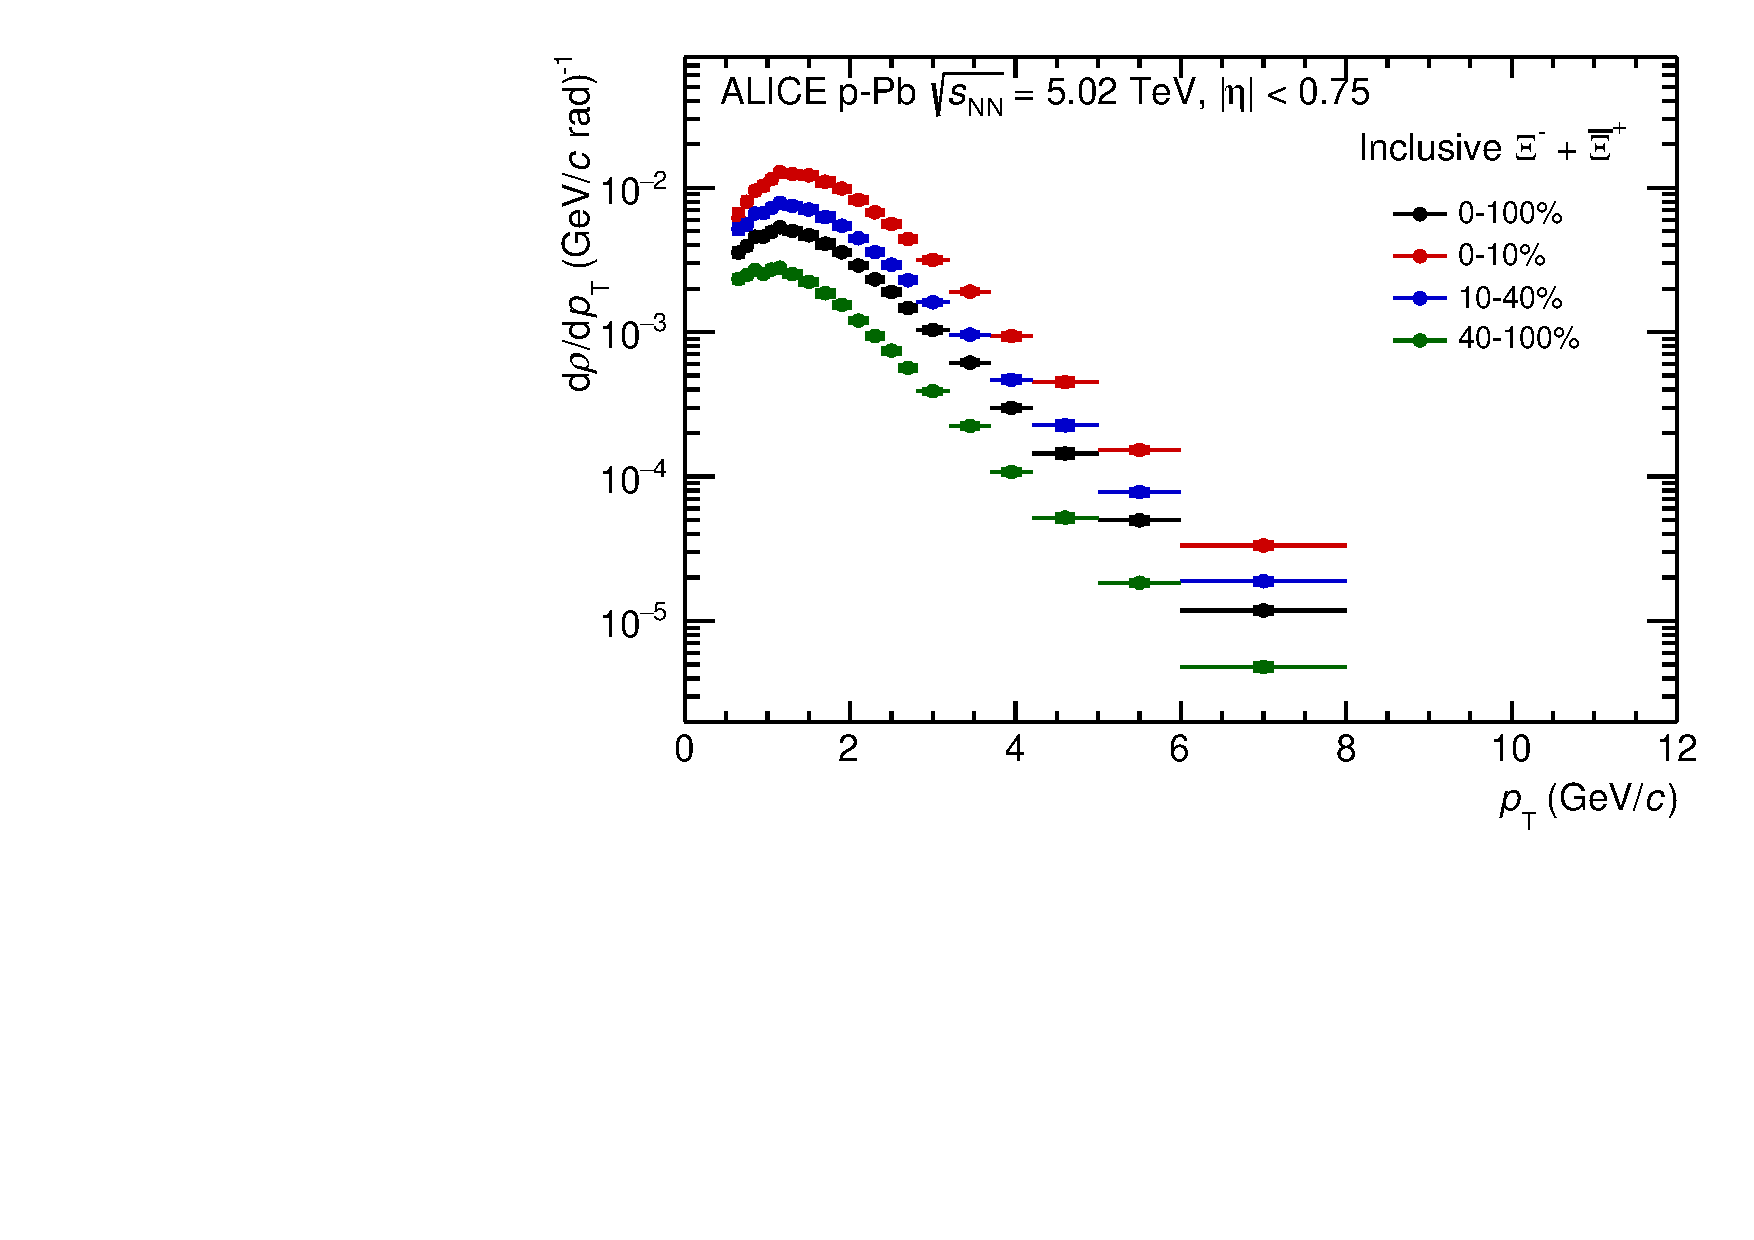
\includegraphics[width=.3\textwidth]{cf6_3}
	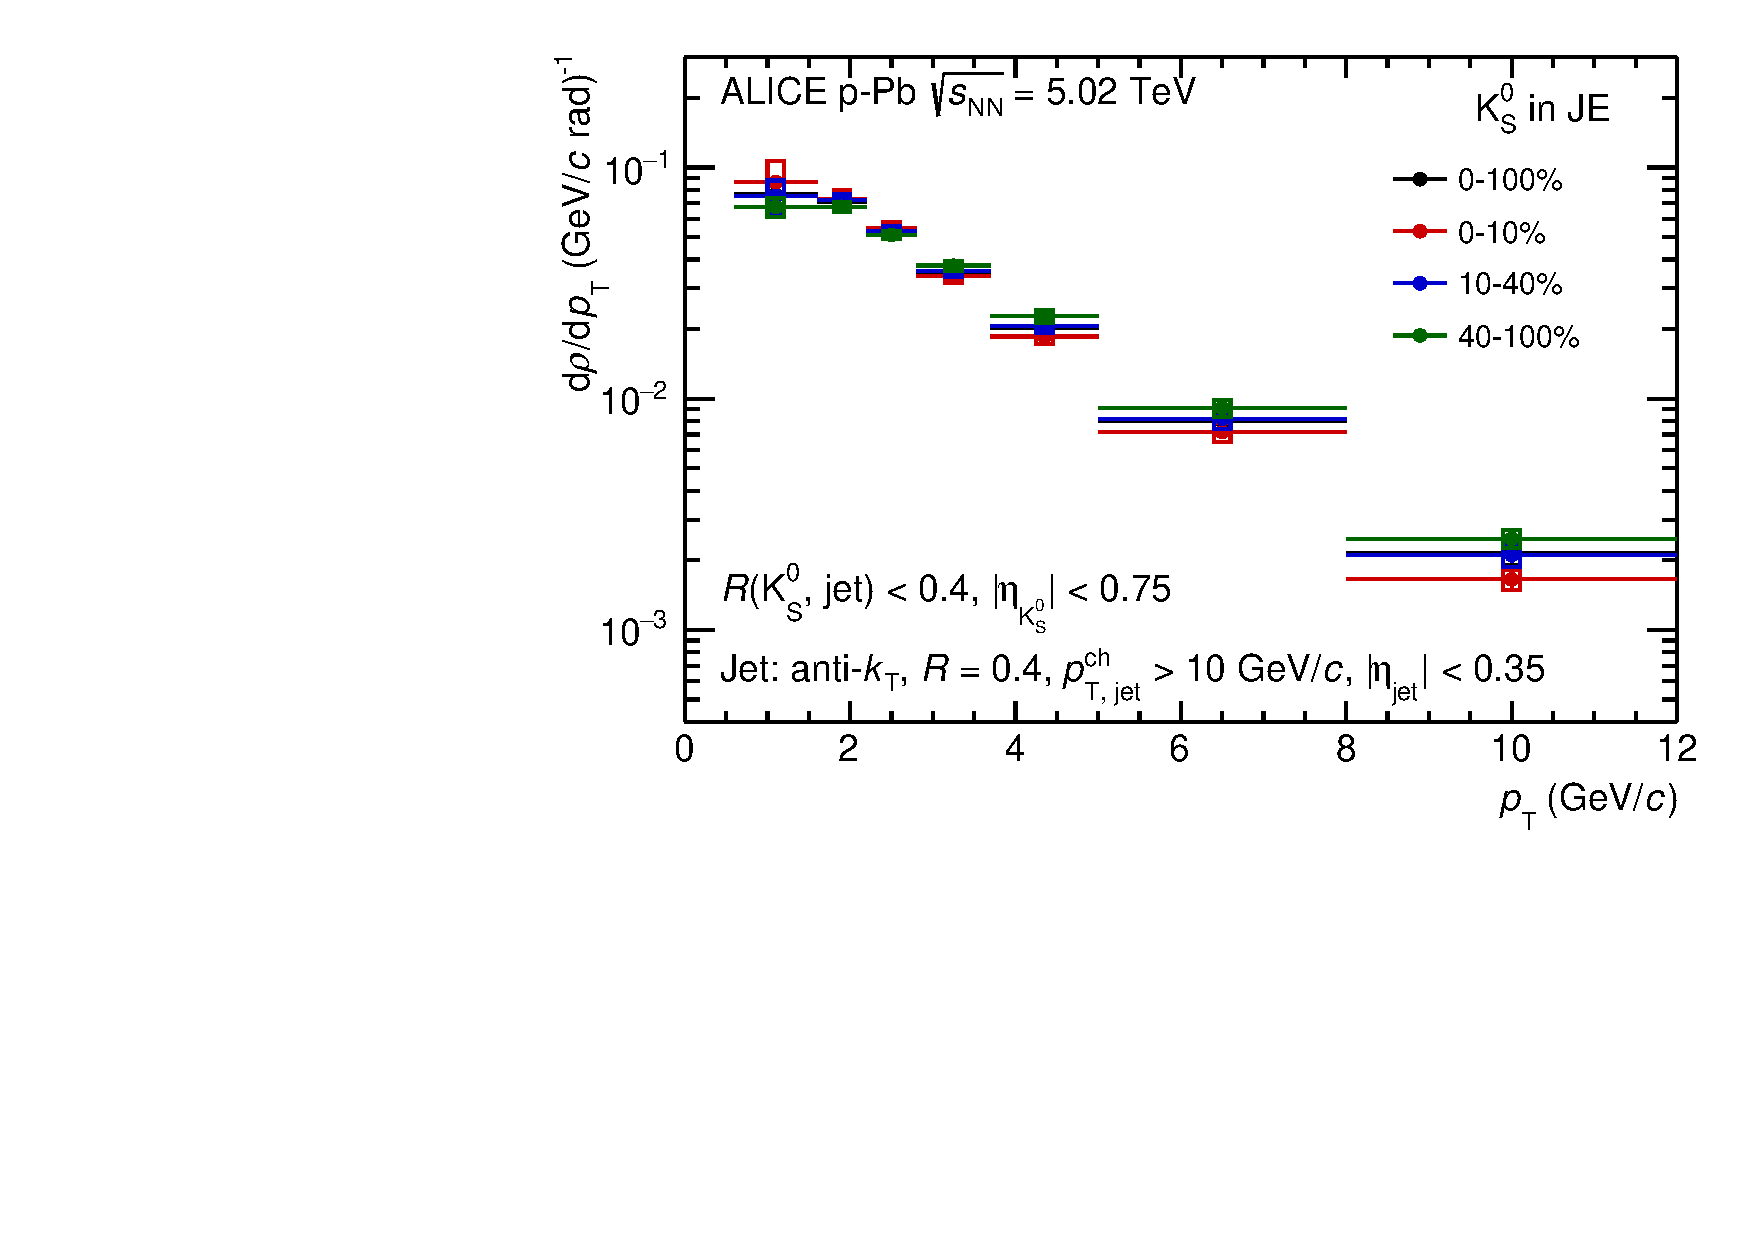
\includegraphics[width=.3\textwidth]{cf6_4}
	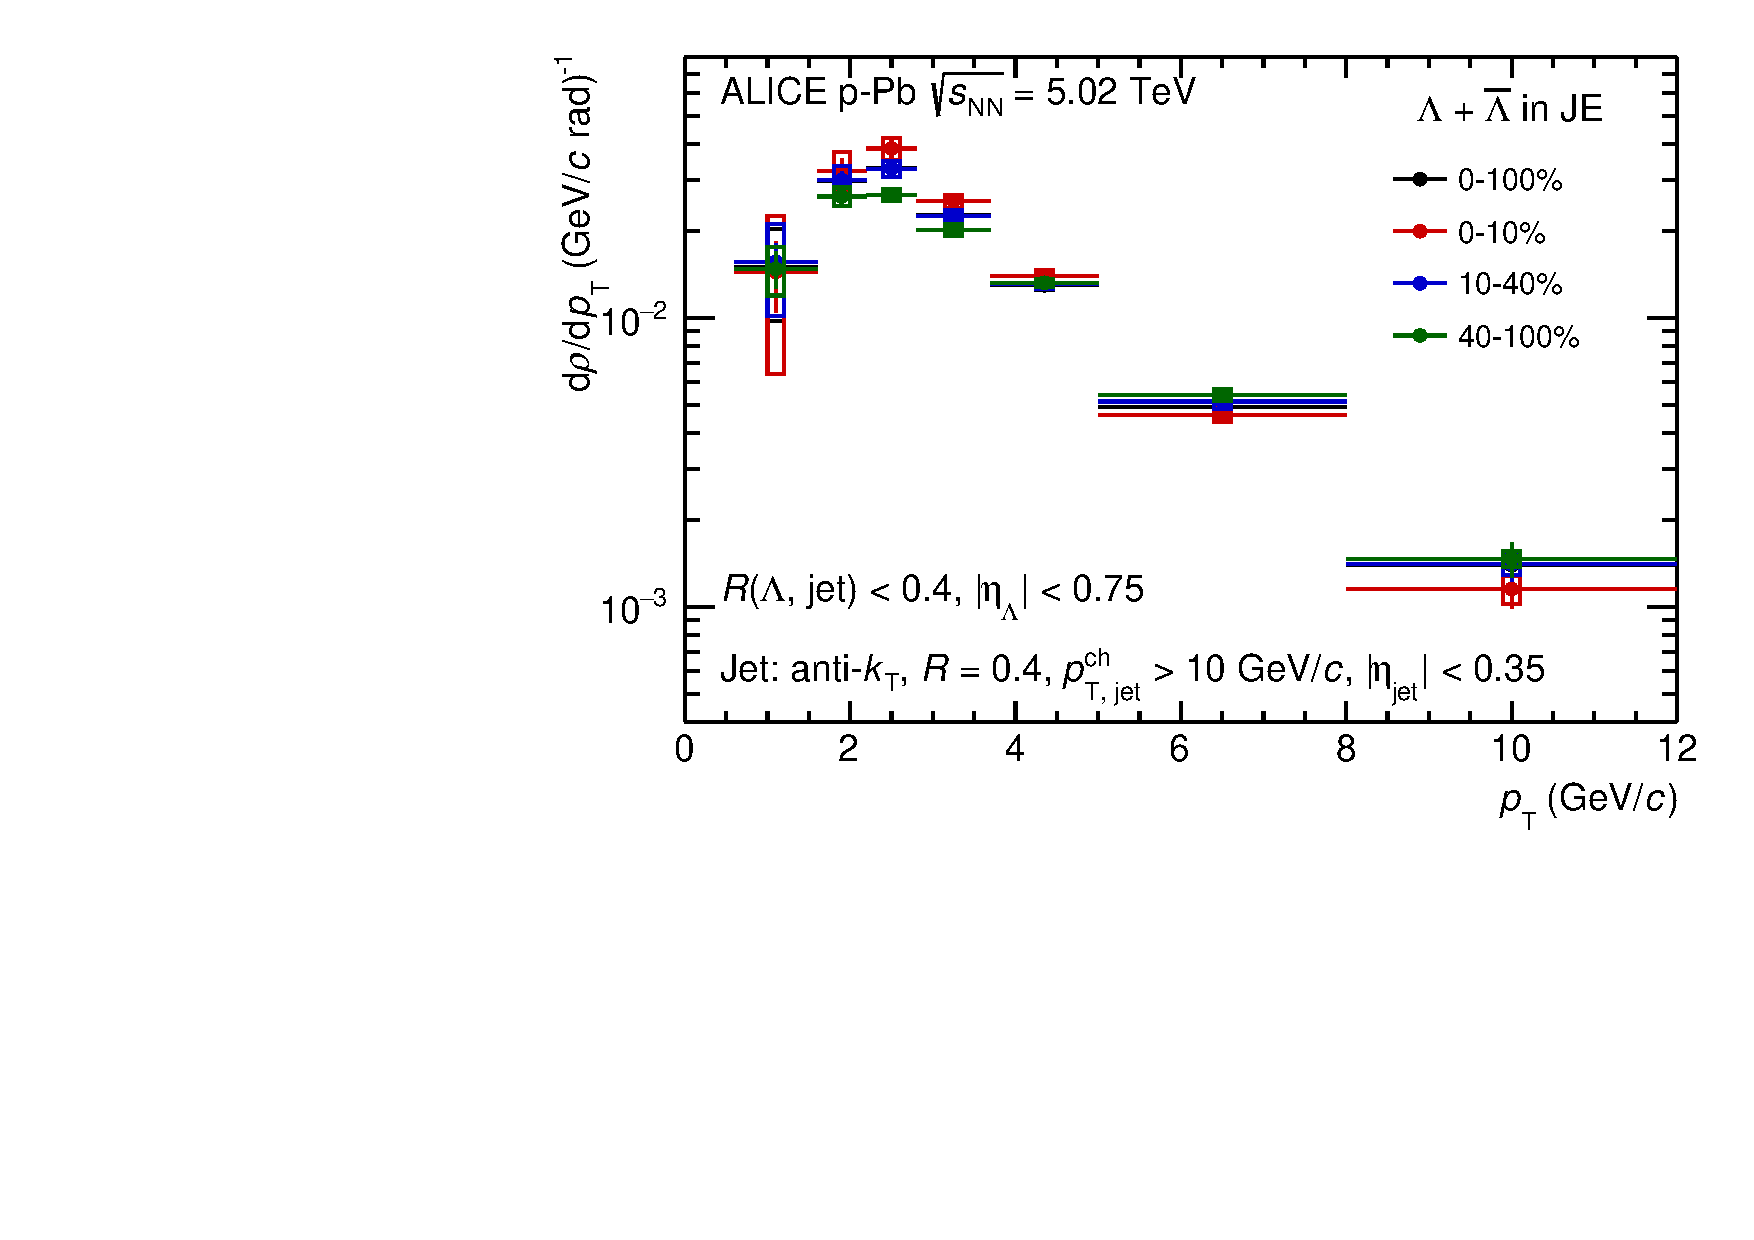
\includegraphics[width=.3\textwidth]{cf6_5}
	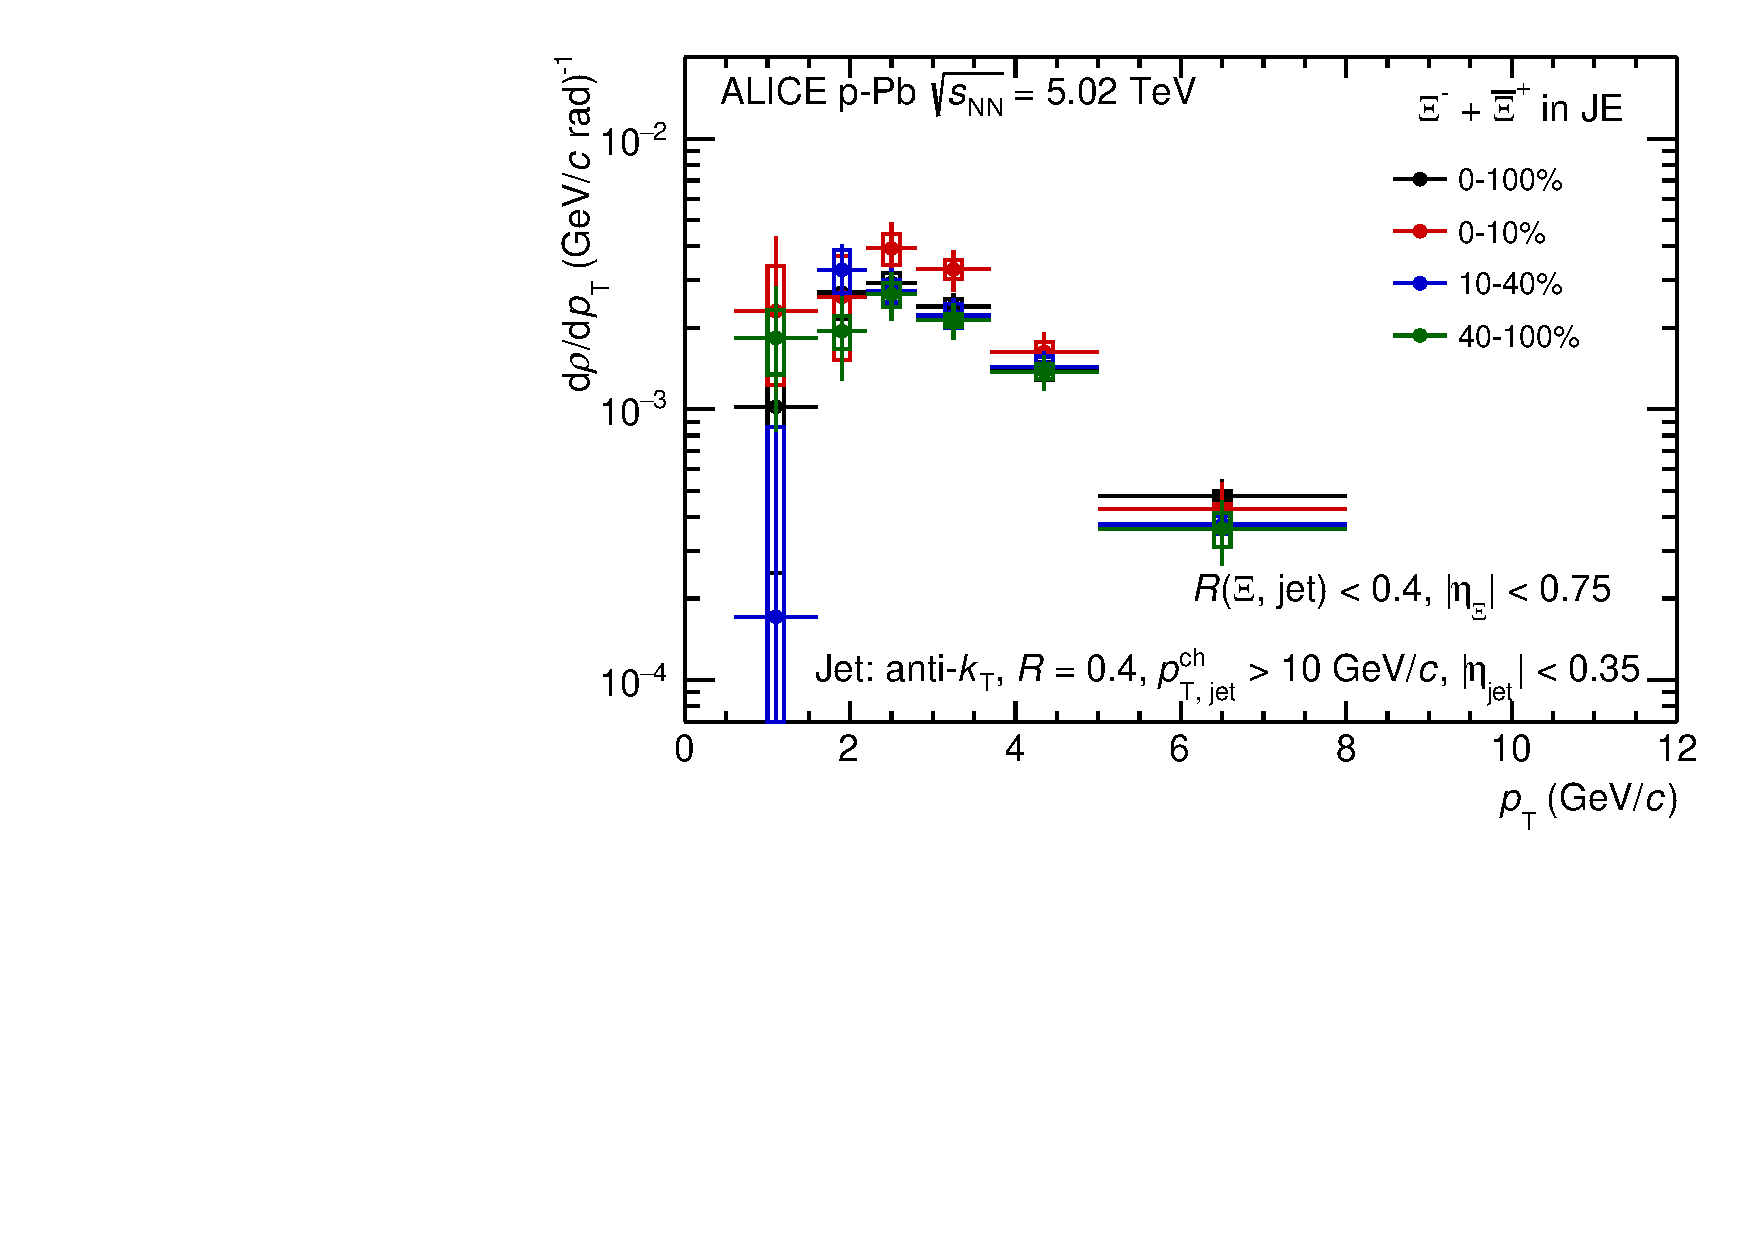
\includegraphics[width=.3\textwidth]{cf6_6}
\end{center}
\caption{$\pT$-differential density of strange hadrons in \pPb in \fivenn within different centrality. }
\label{fig:pPbSpectwCent}
\end{figure}
\subsection{Baryon-to-meson and baryon-to-baryon ratios}
\label{subsec:ParRatios}
\begin{figure}[!ht]
	\begin{center}
		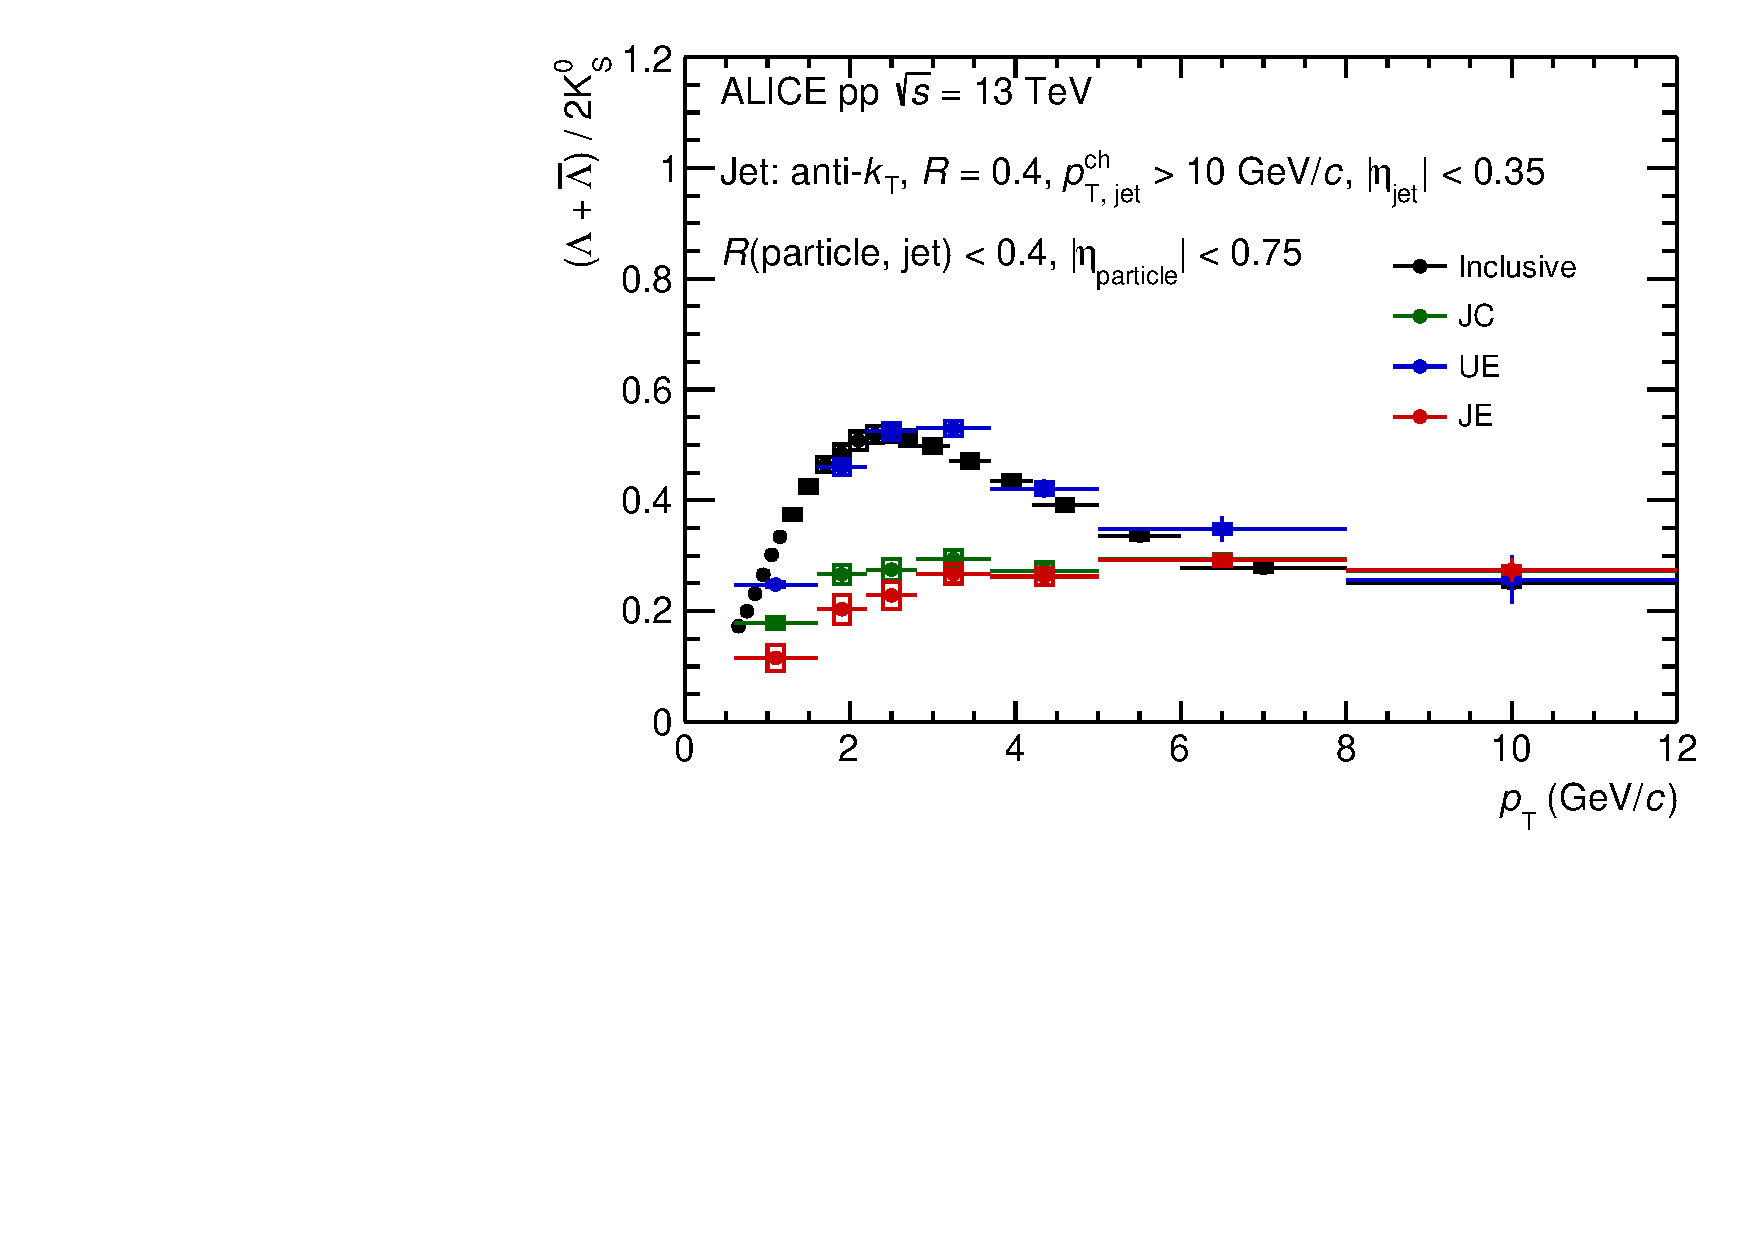
\includegraphics[width=.3\textwidth]{cf7_1}
		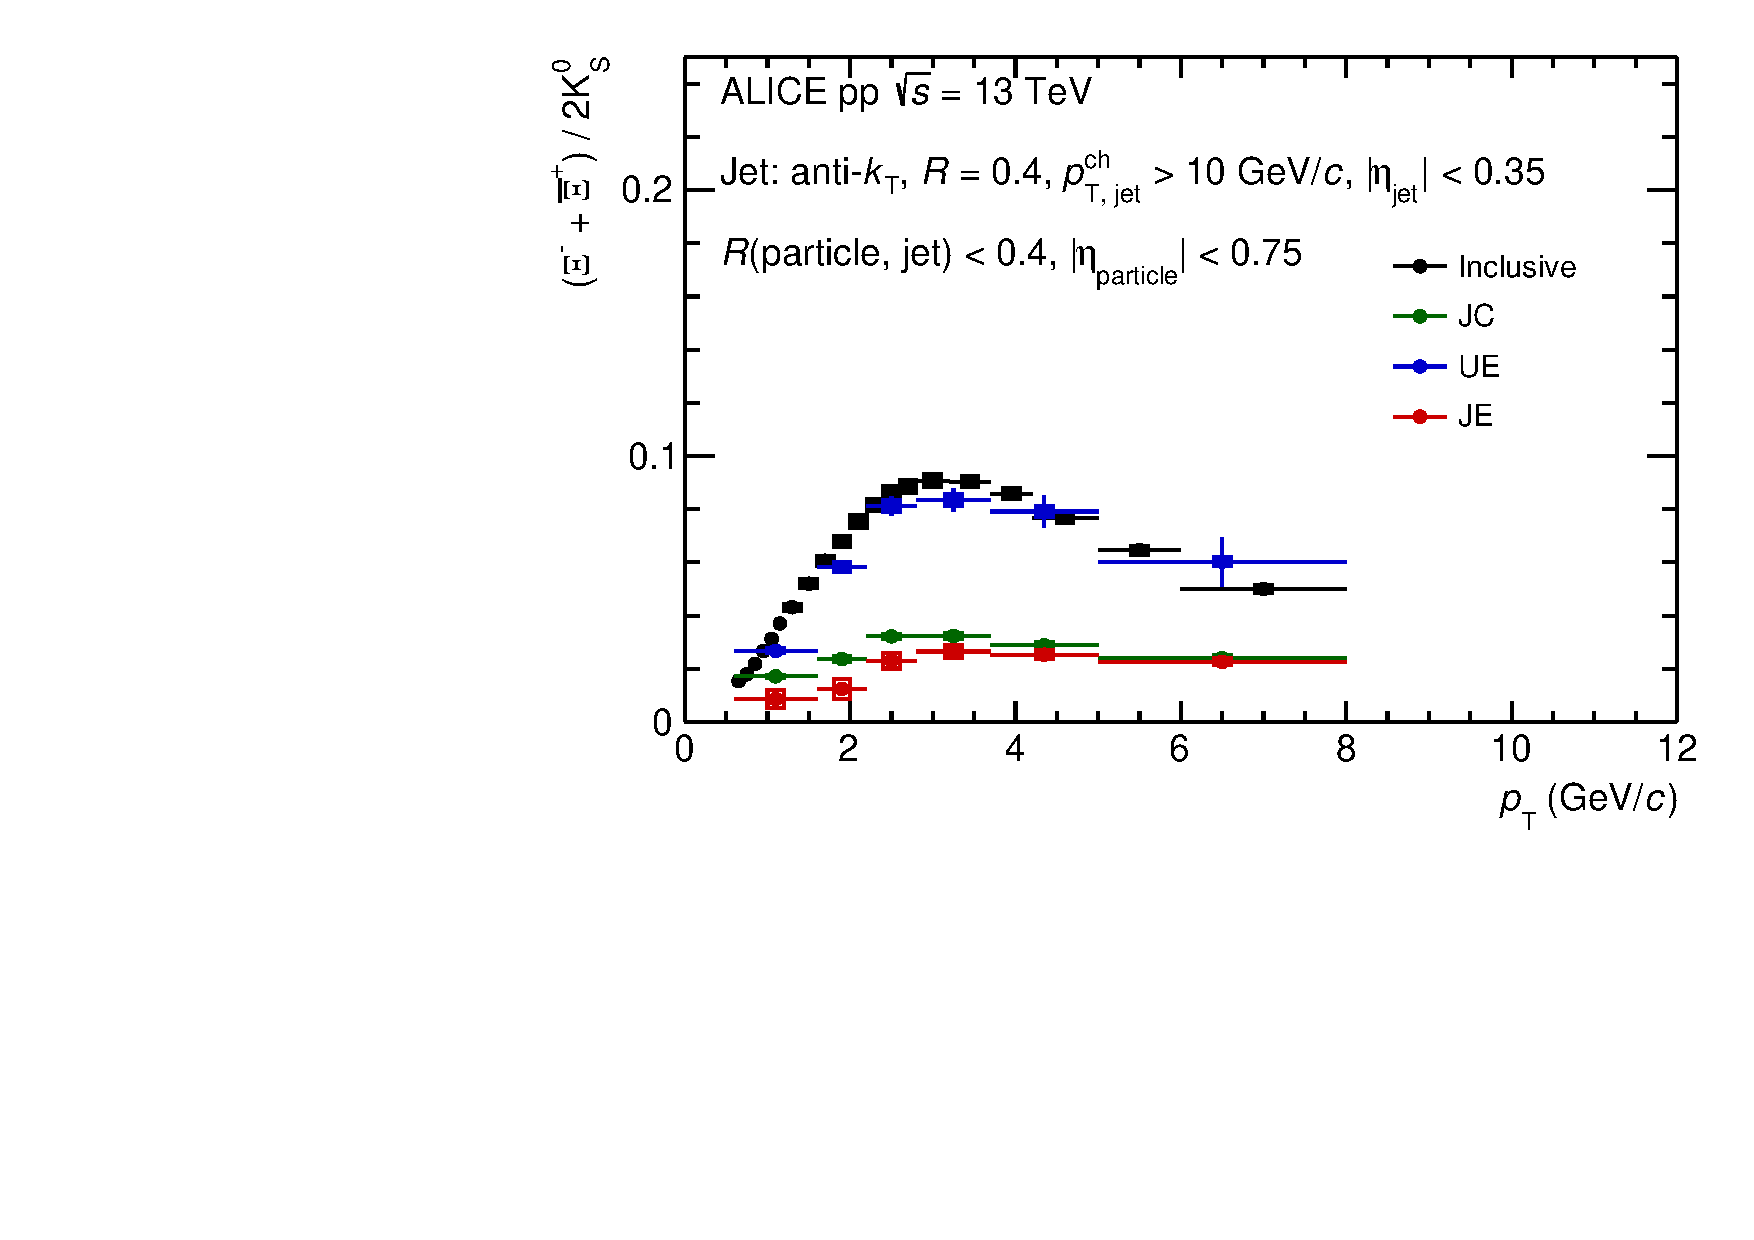
\includegraphics[width=.3\textwidth]{cf7_2}
		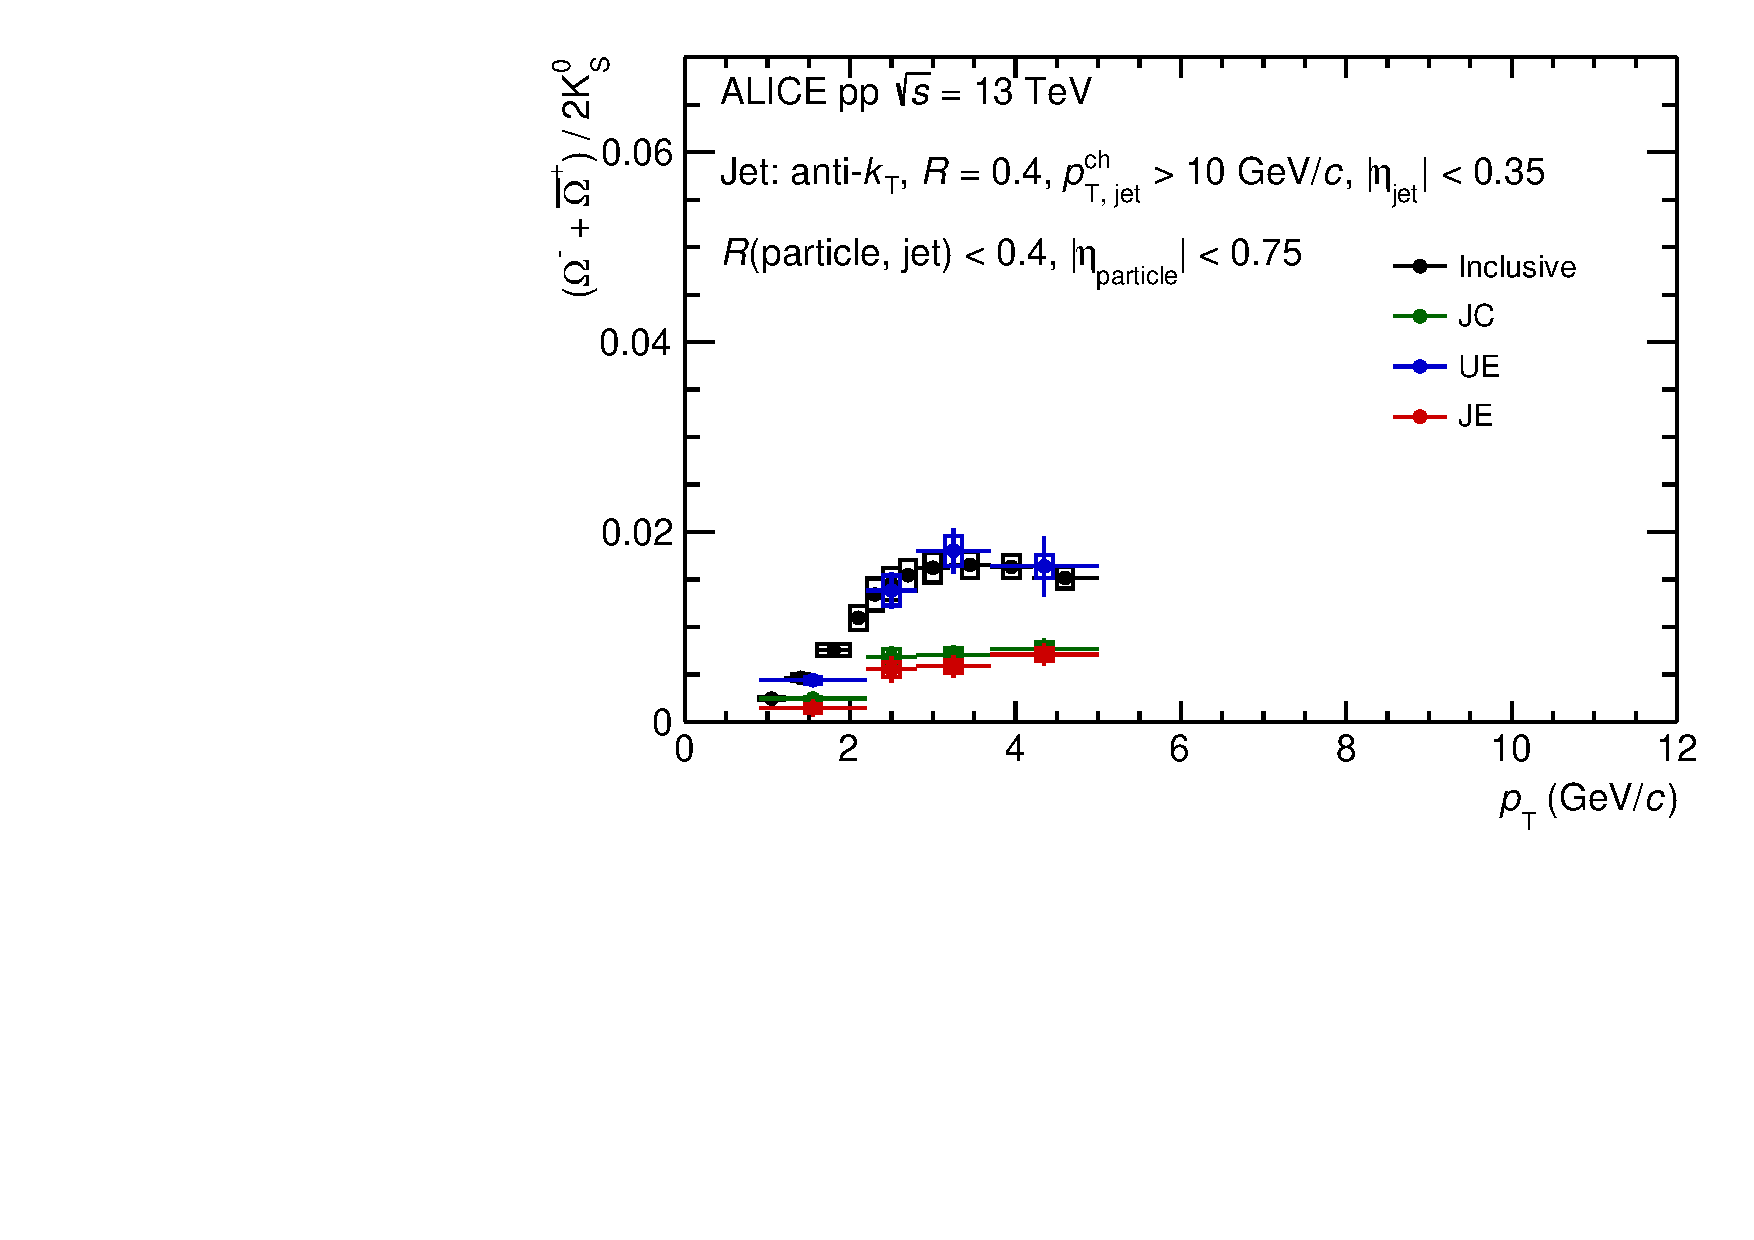
\includegraphics[width=.3\textwidth]{cf7_3}
		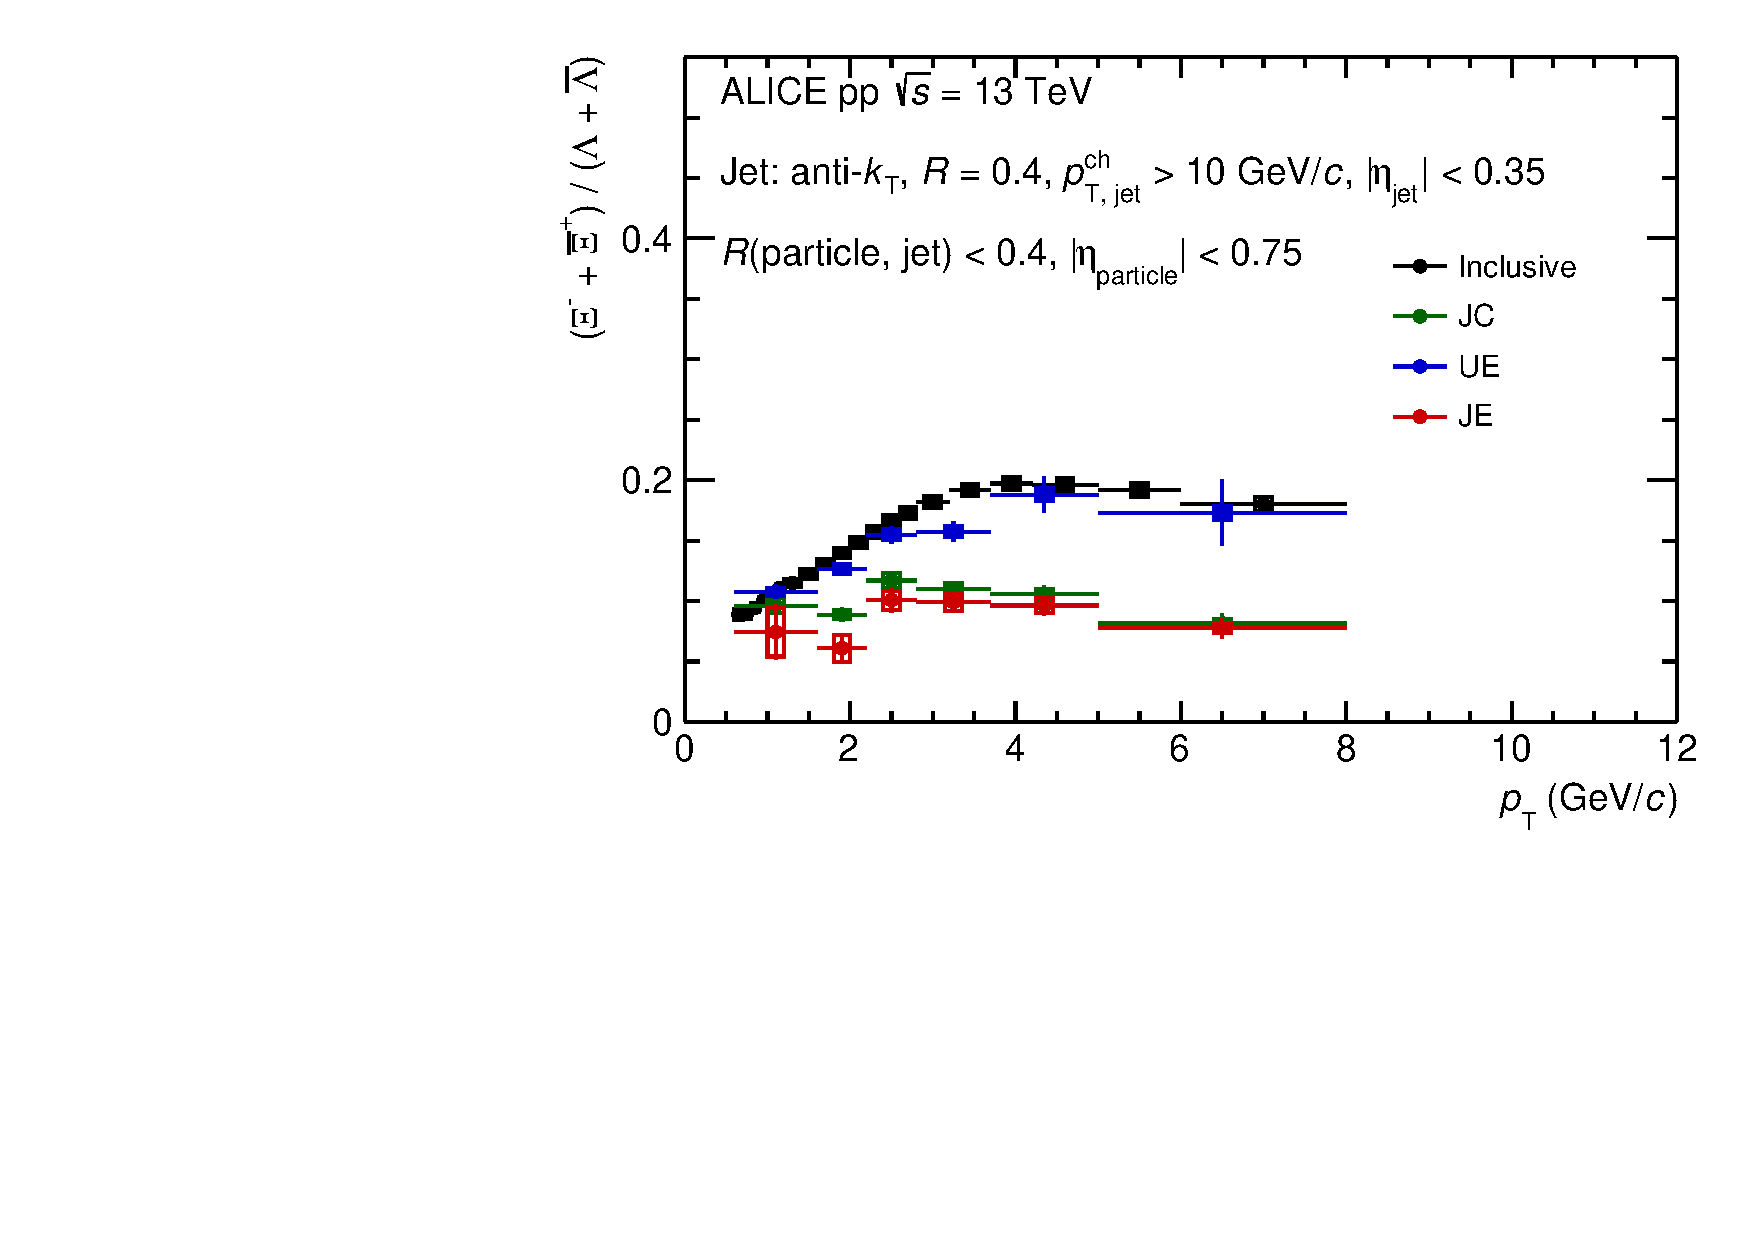
\includegraphics[width=.3\textwidth]{cf7_4}
		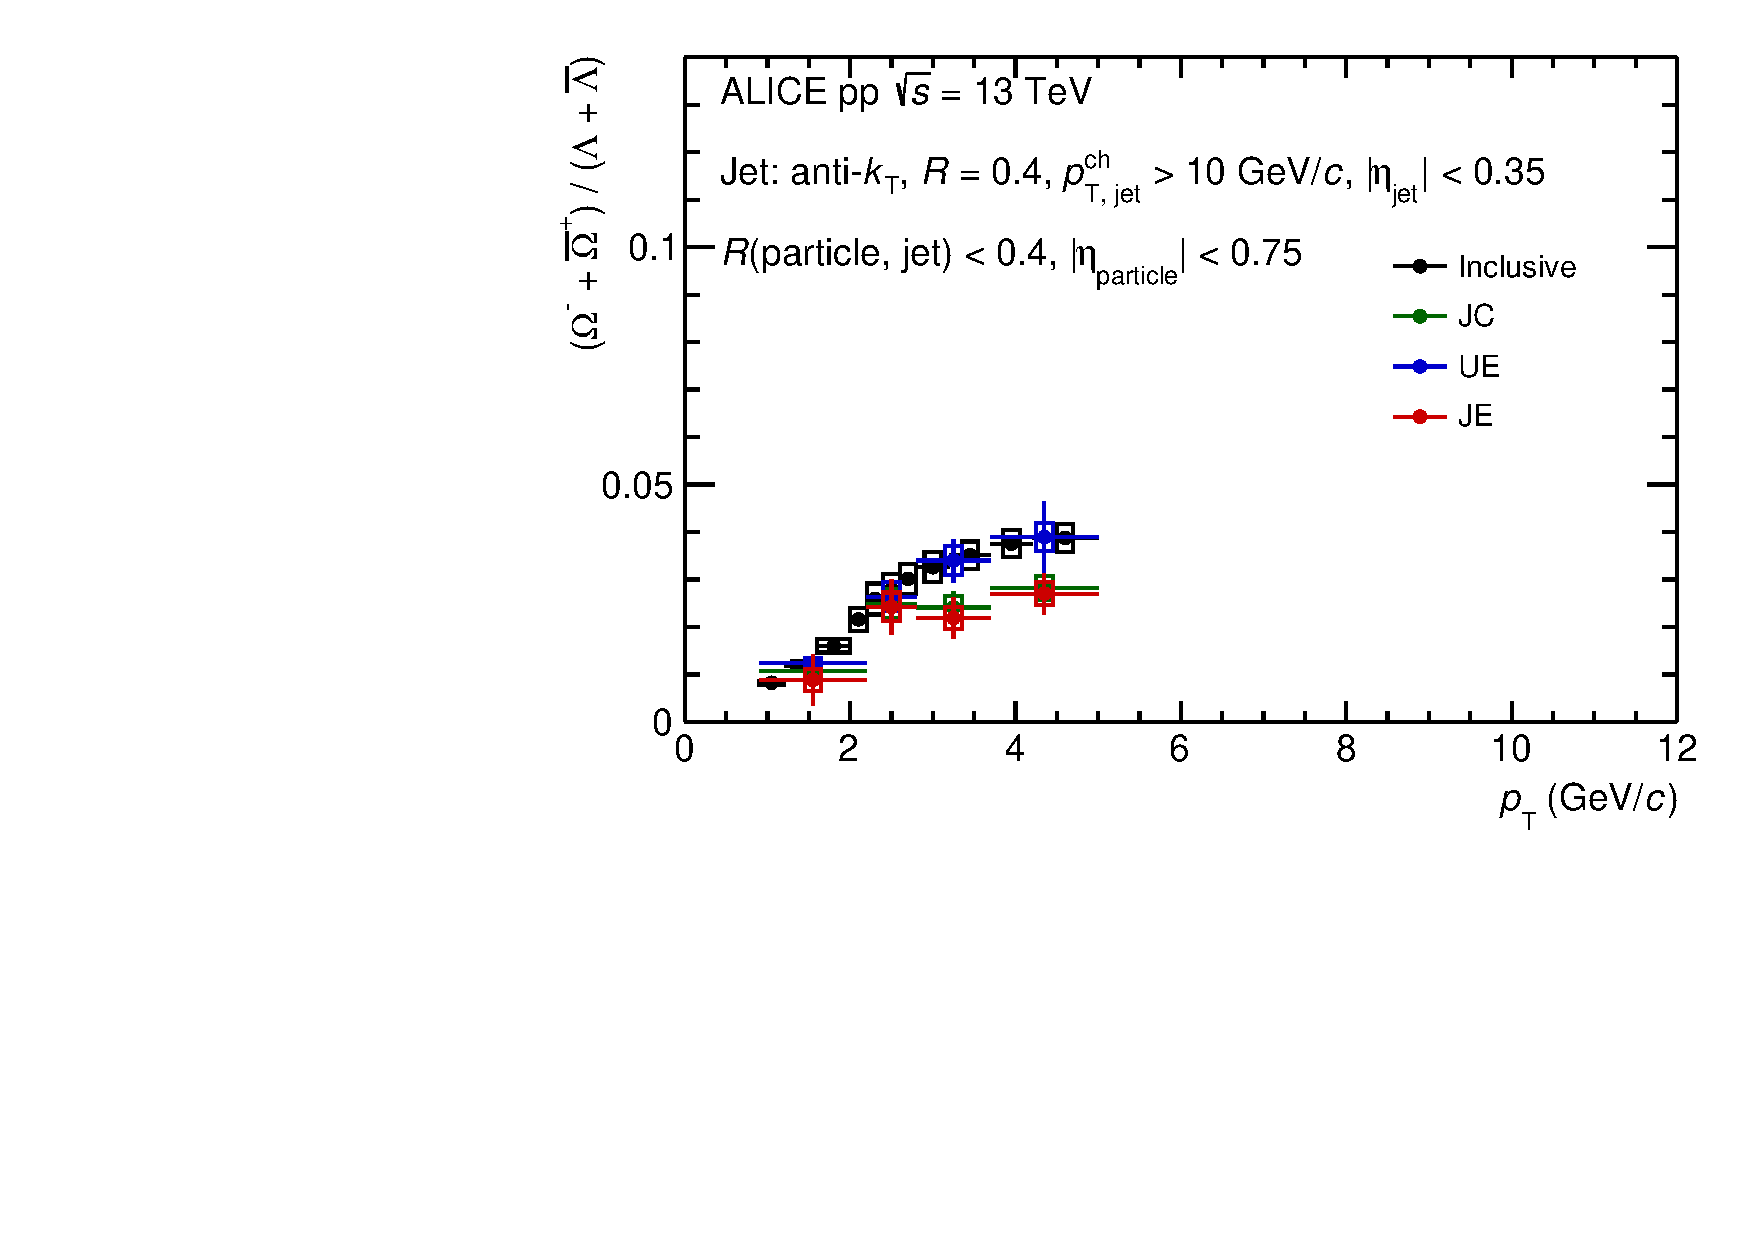
\includegraphics[width=.3\textwidth]{cf7_5}
		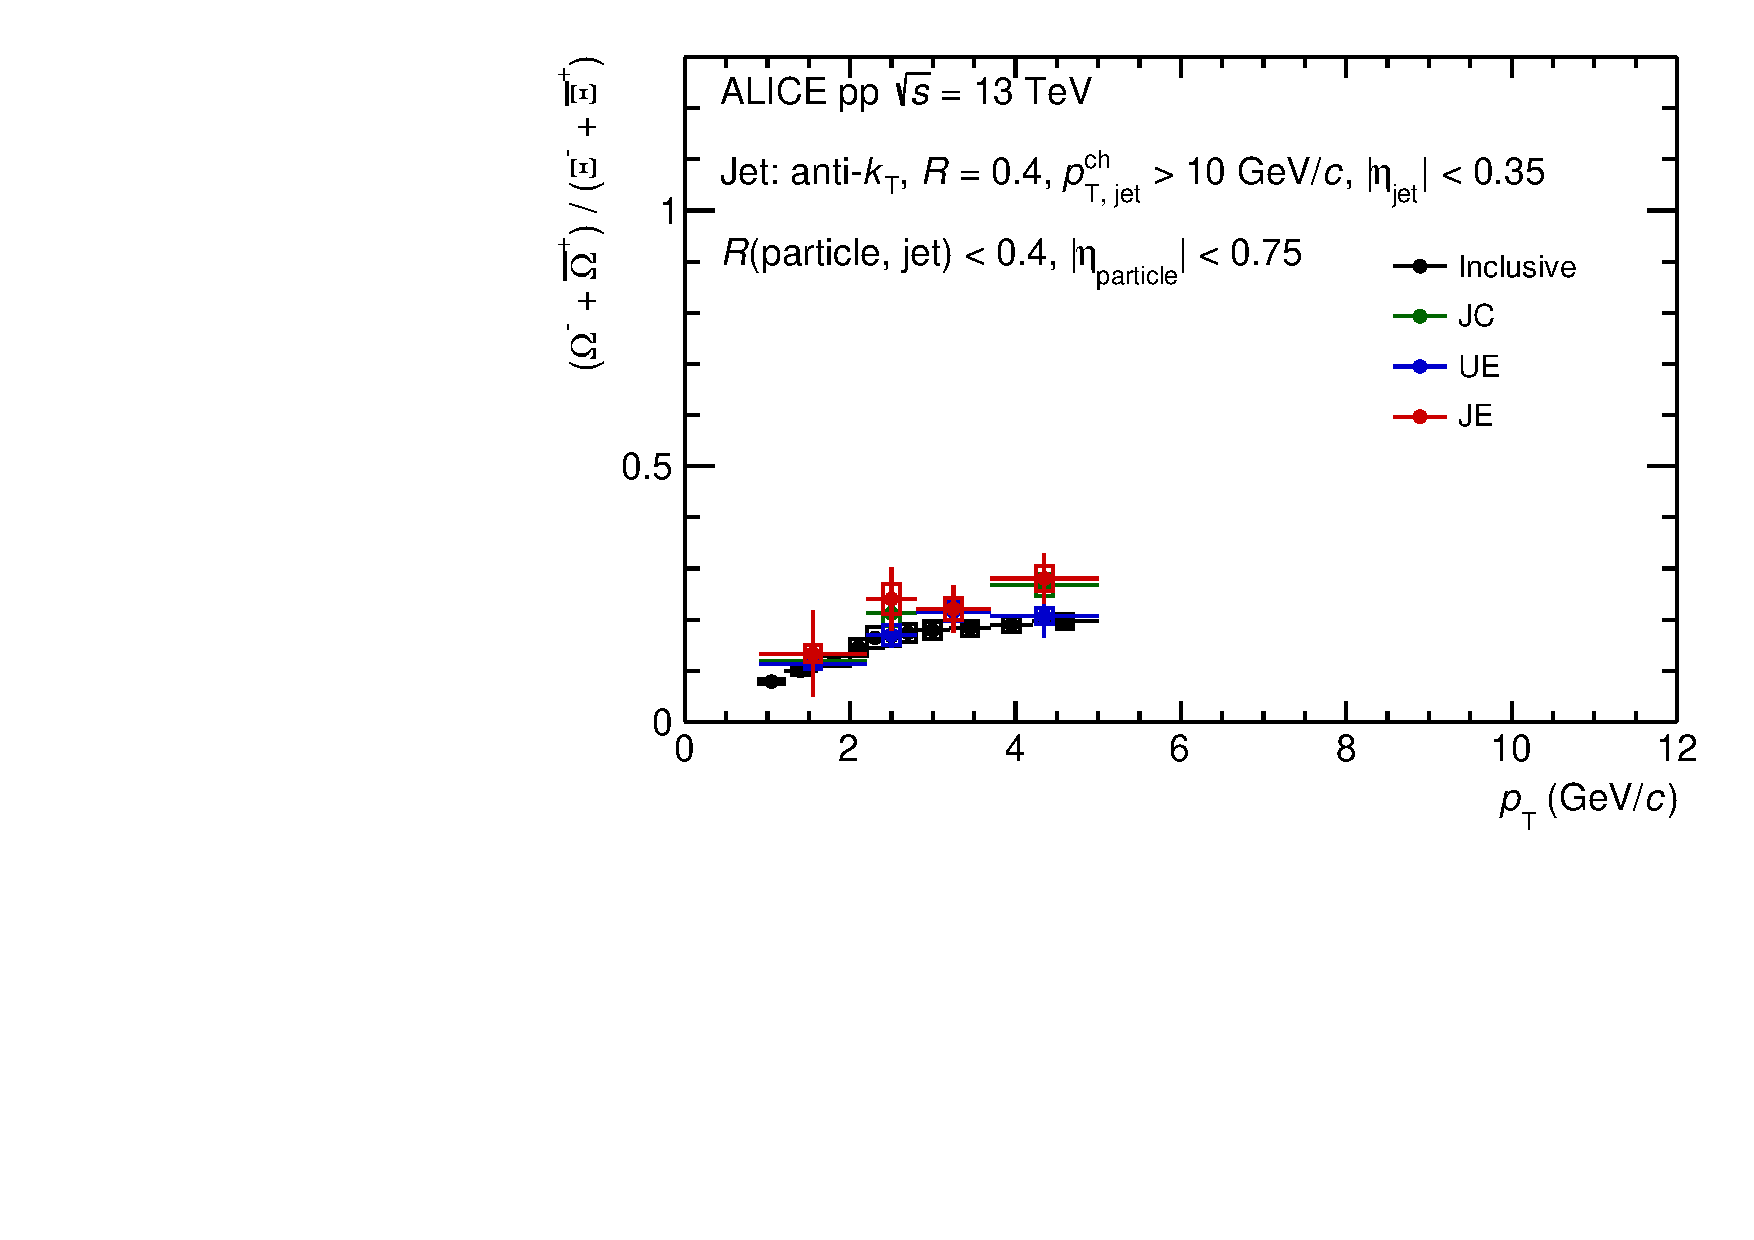
\includegraphics[width=.3\textwidth]{cf7_6}
	\end{center}
	\caption{Particle ratios.}
	\label{fig:ppRatio}
\end{figure}
\begin{figure}[!ht]
	\begin{center}
		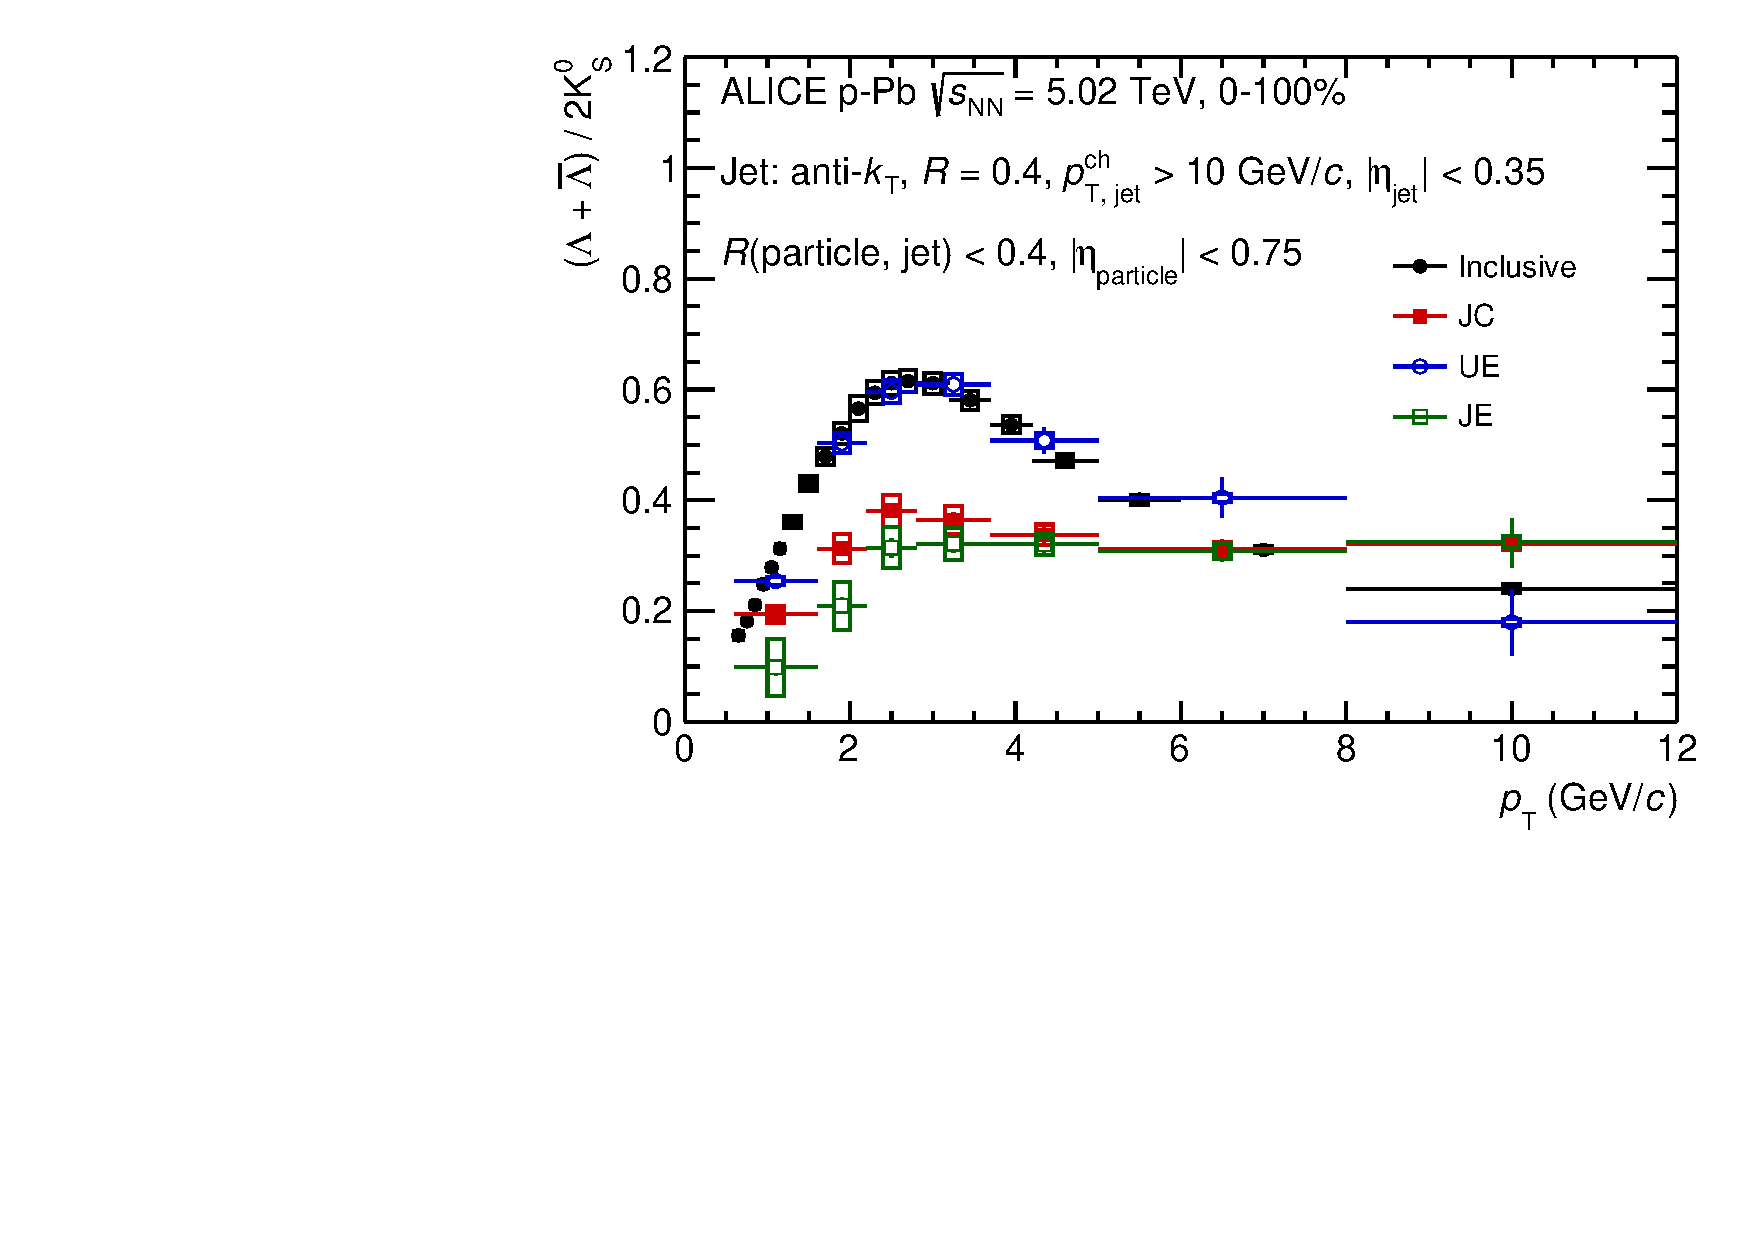
\includegraphics[width=.3\textwidth]{cf8_1}
		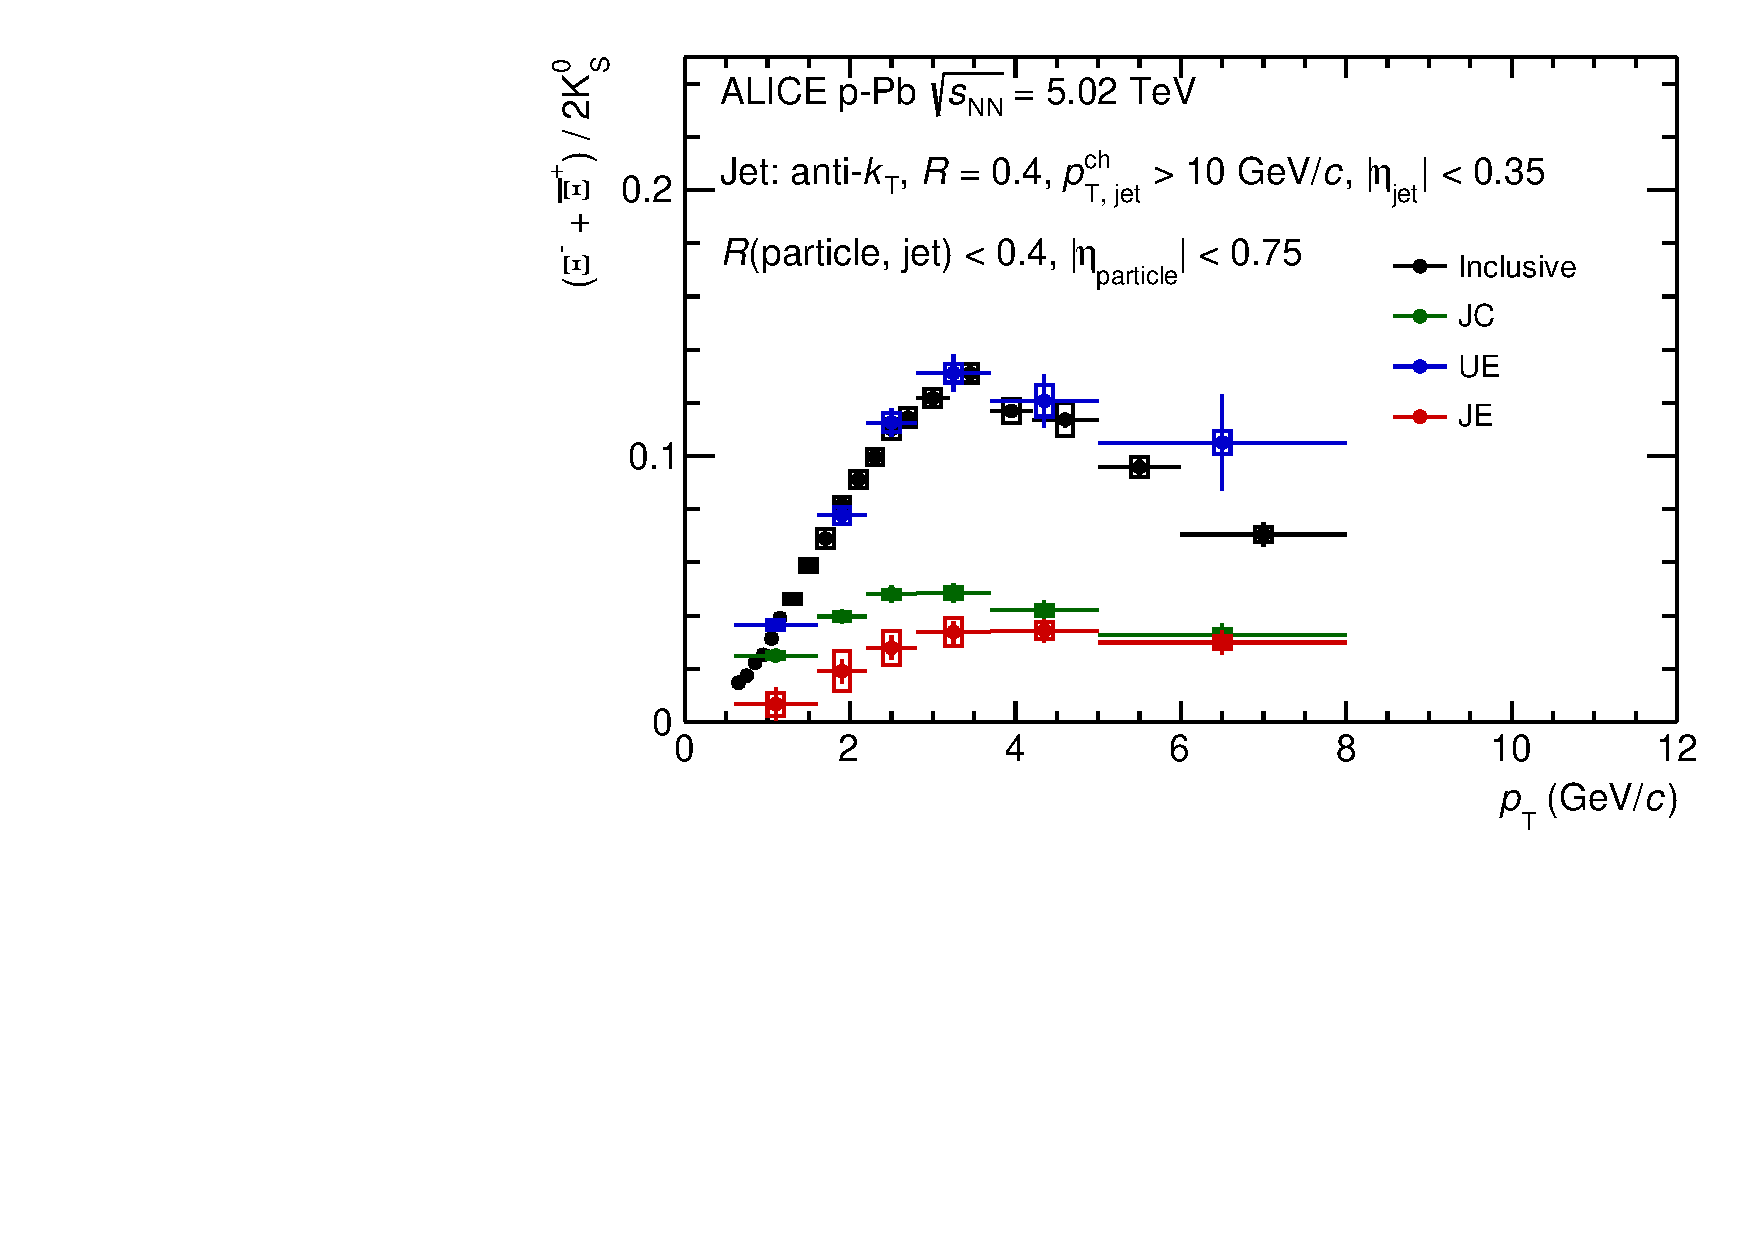
\includegraphics[width=.3\textwidth]{cf8_2}
		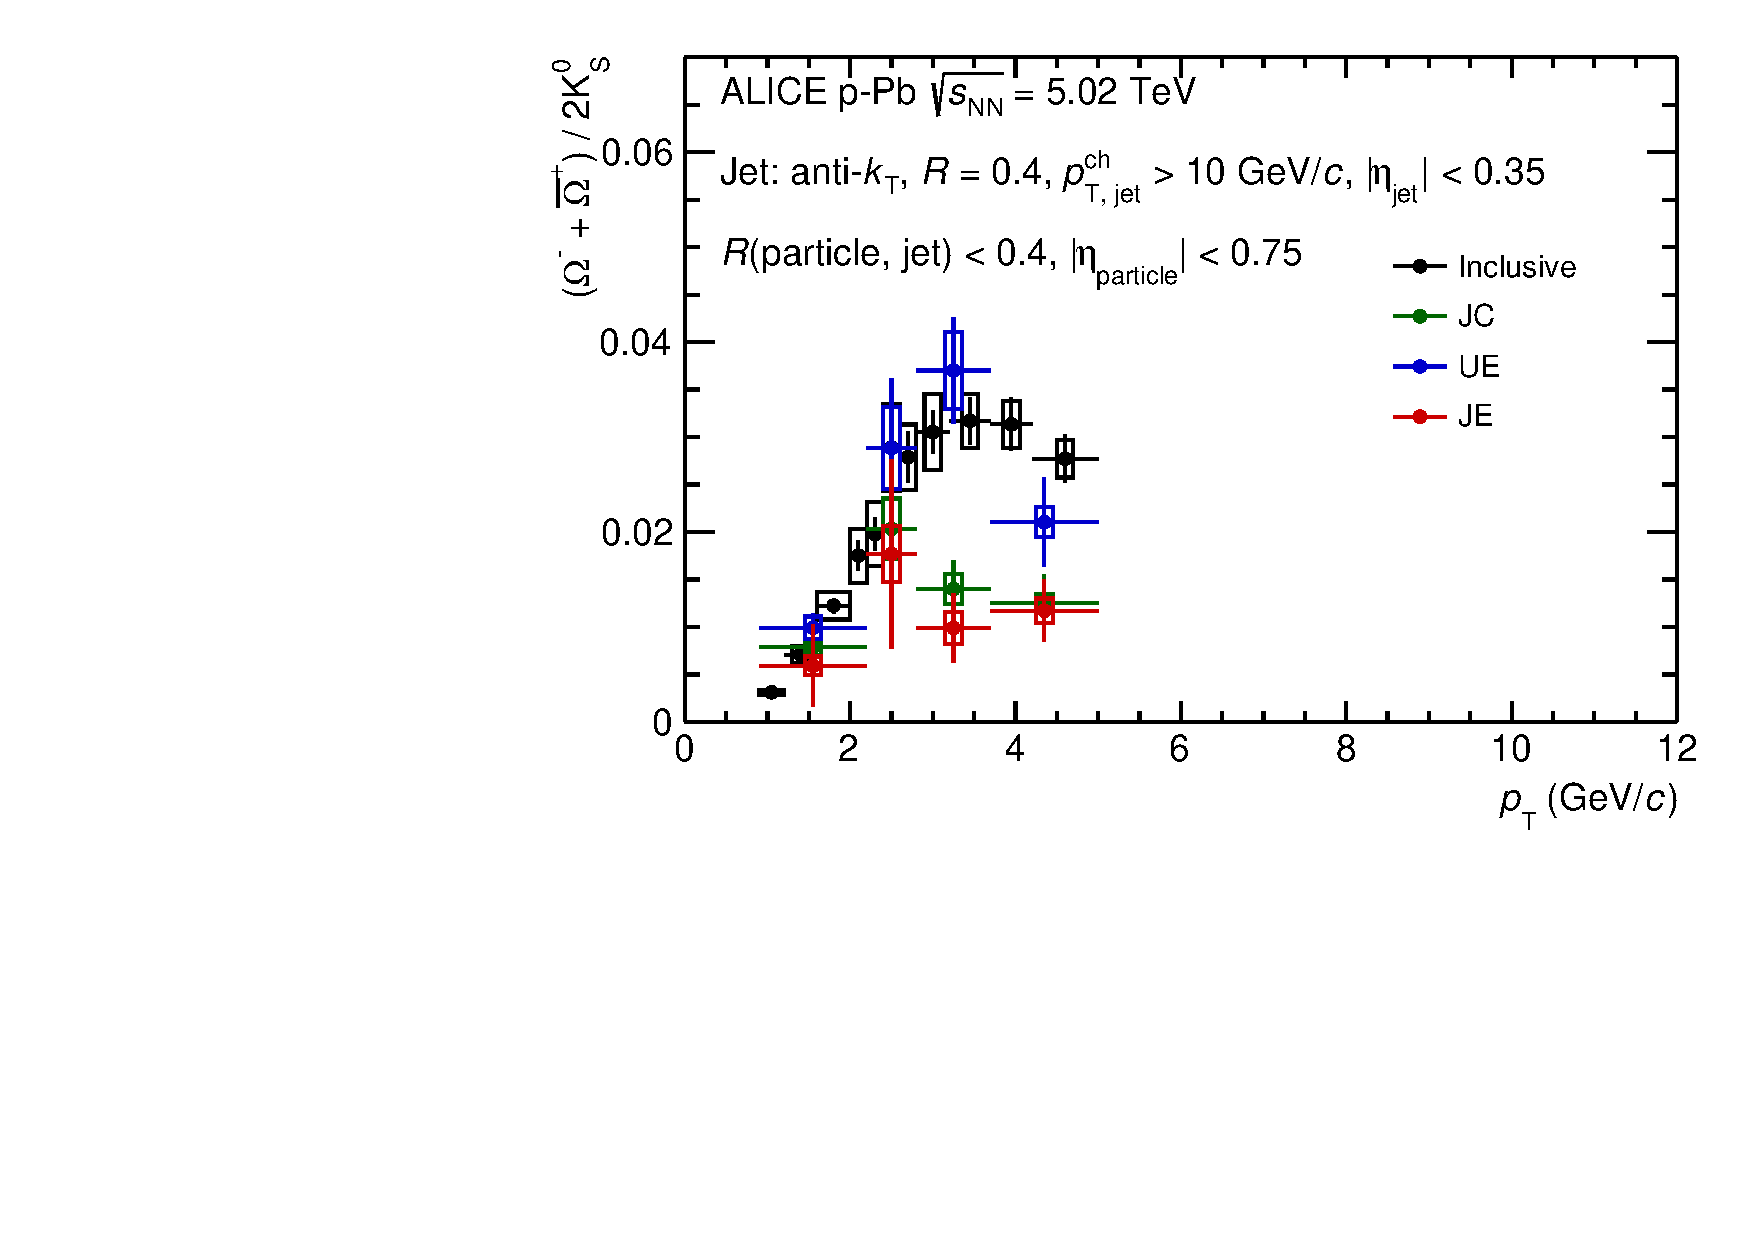
\includegraphics[width=.3\textwidth]{cf8_3}
		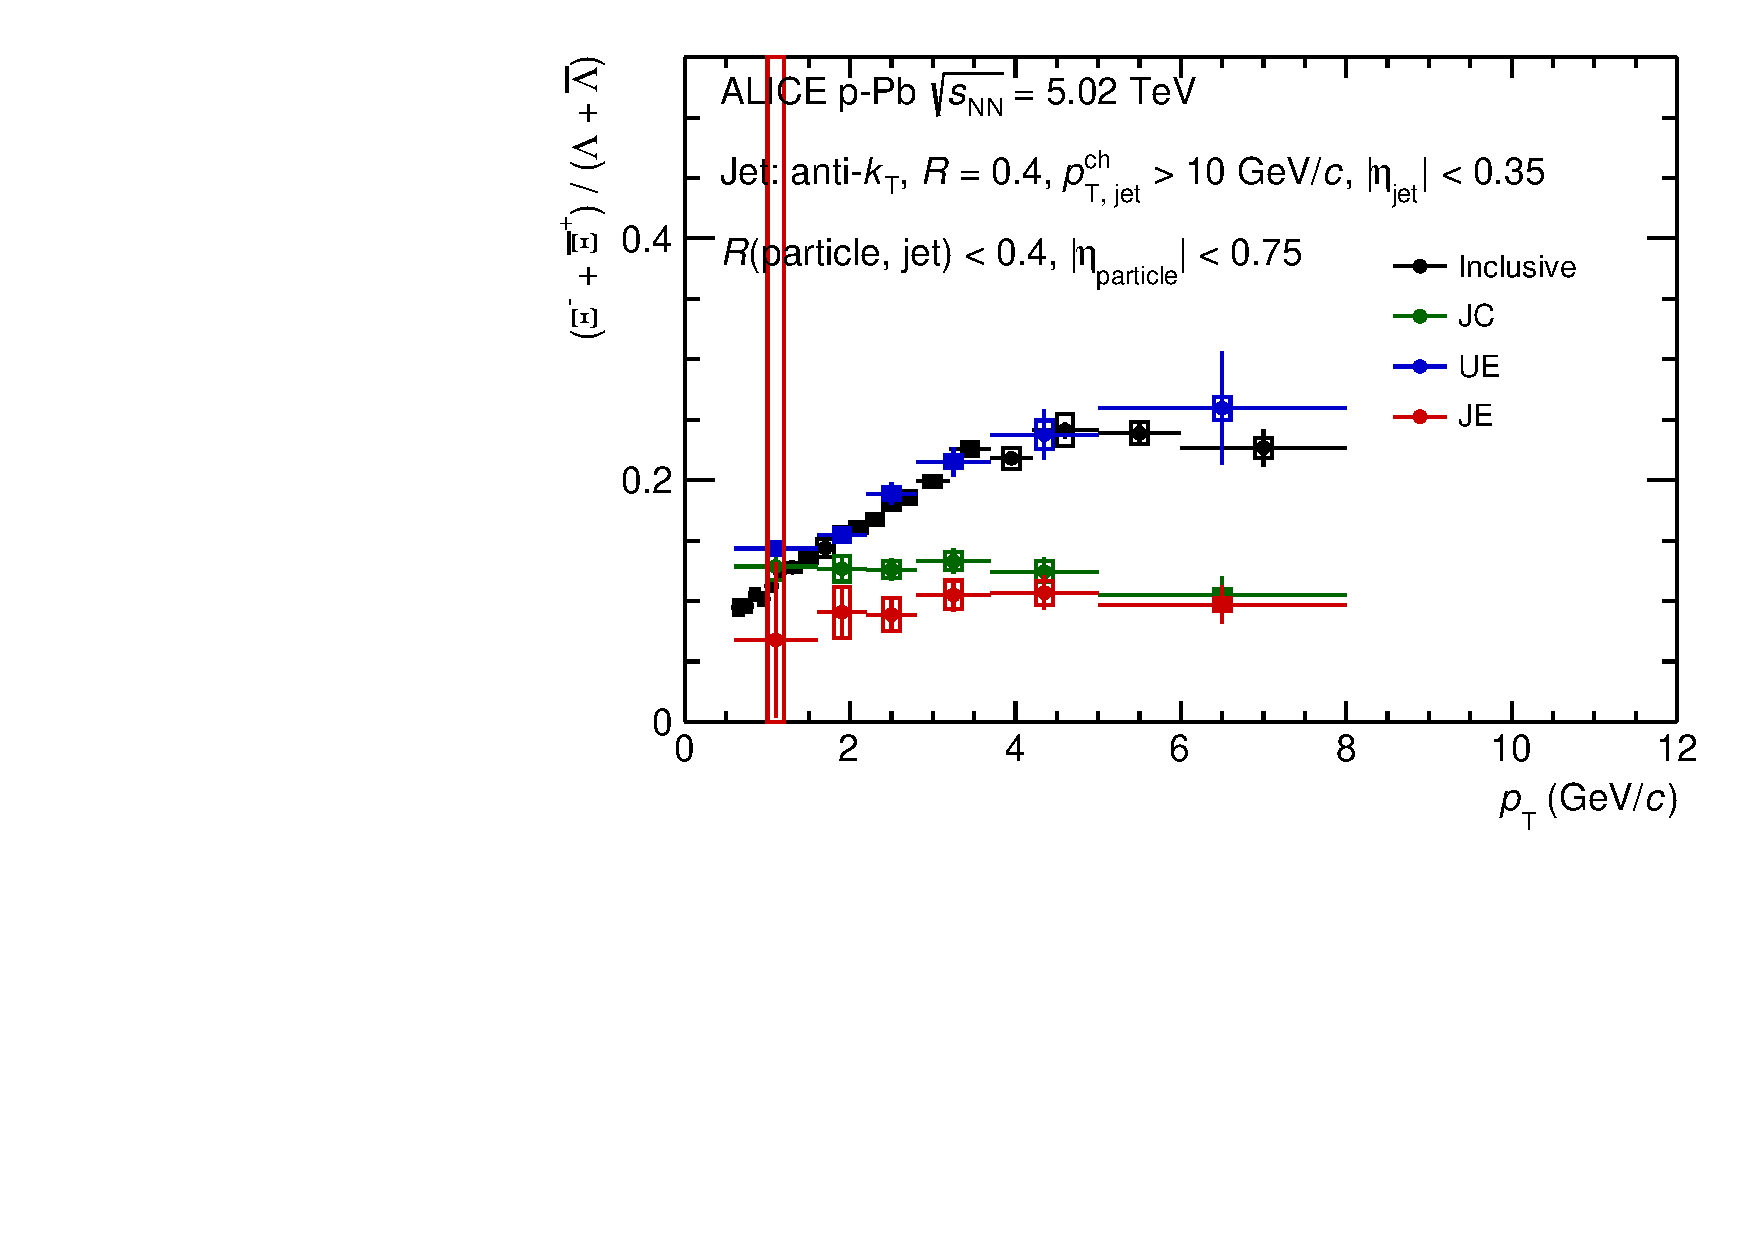
\includegraphics[width=.3\textwidth]{cf8_4}
		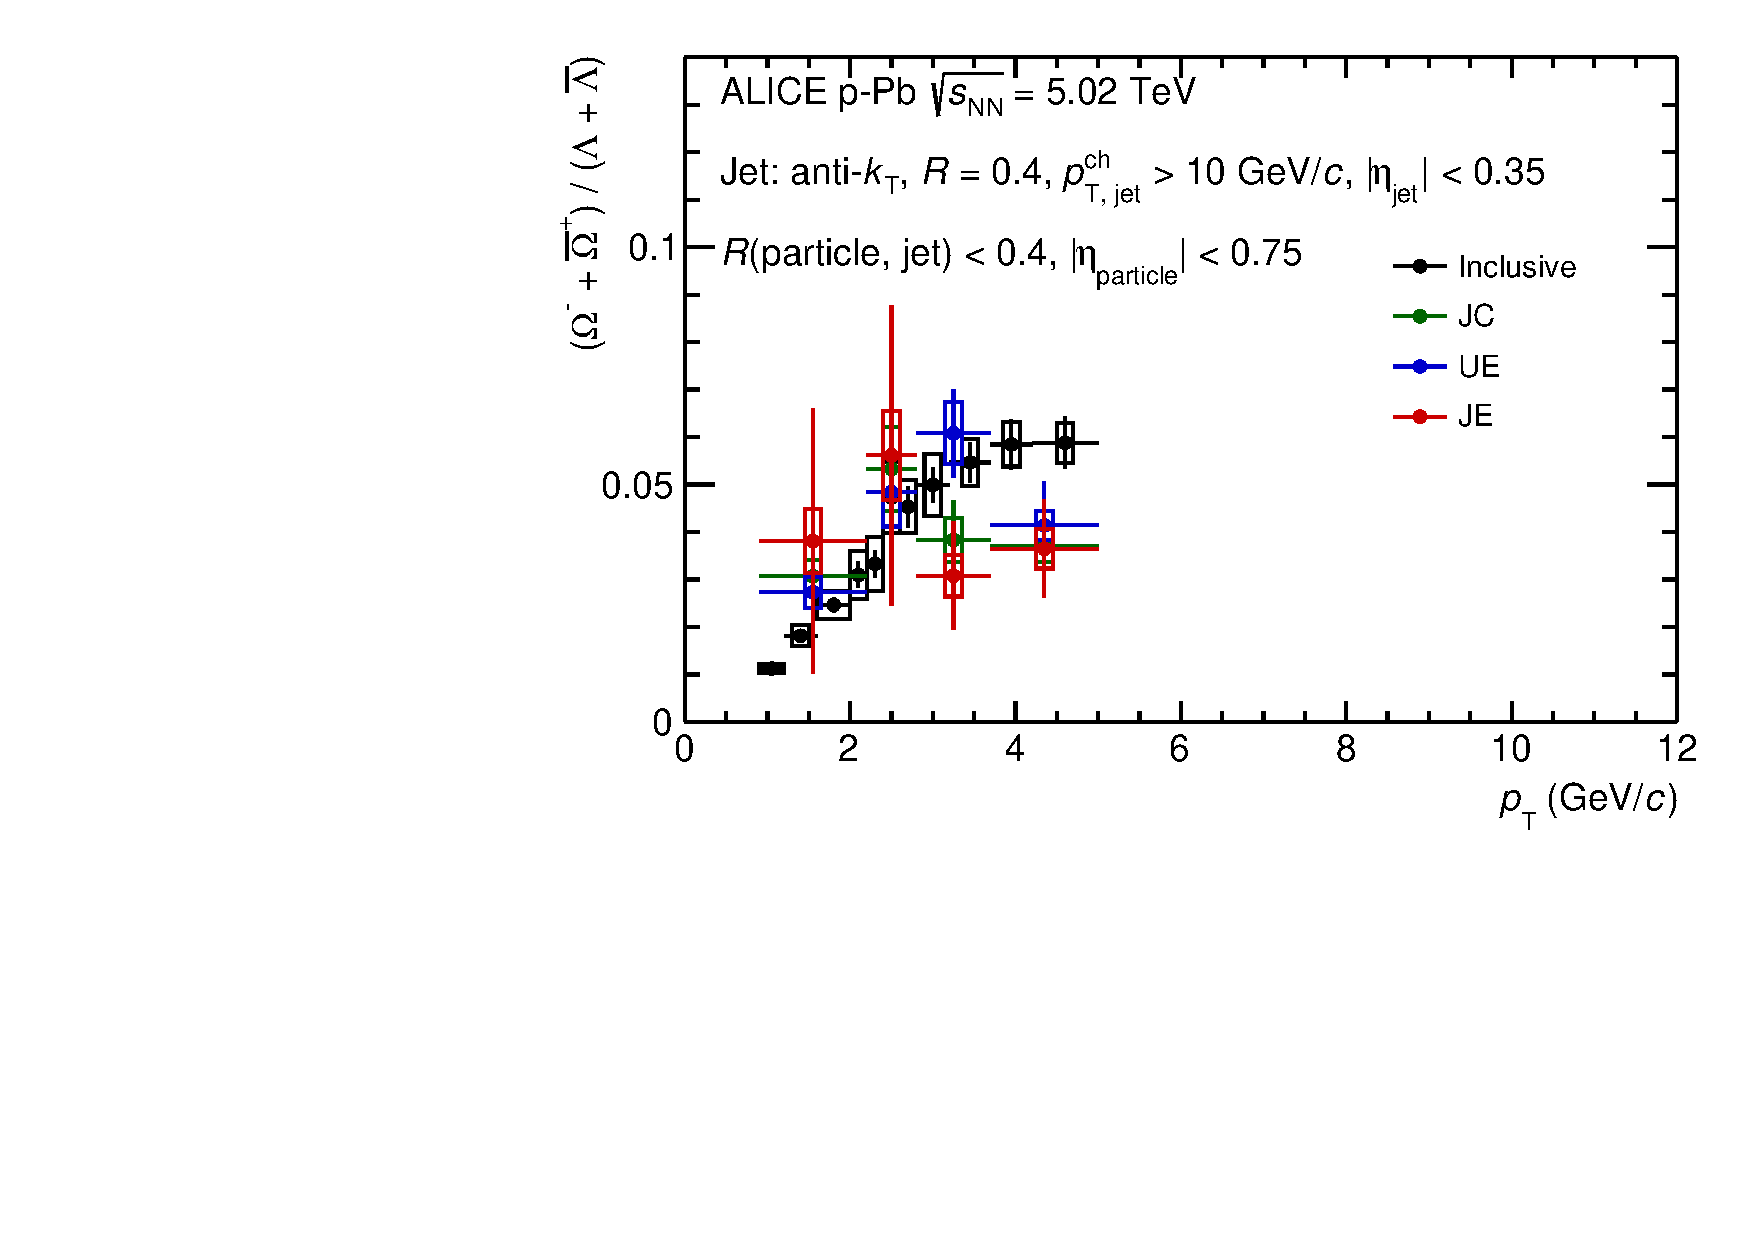
\includegraphics[width=.3\textwidth]{cf8_5}
		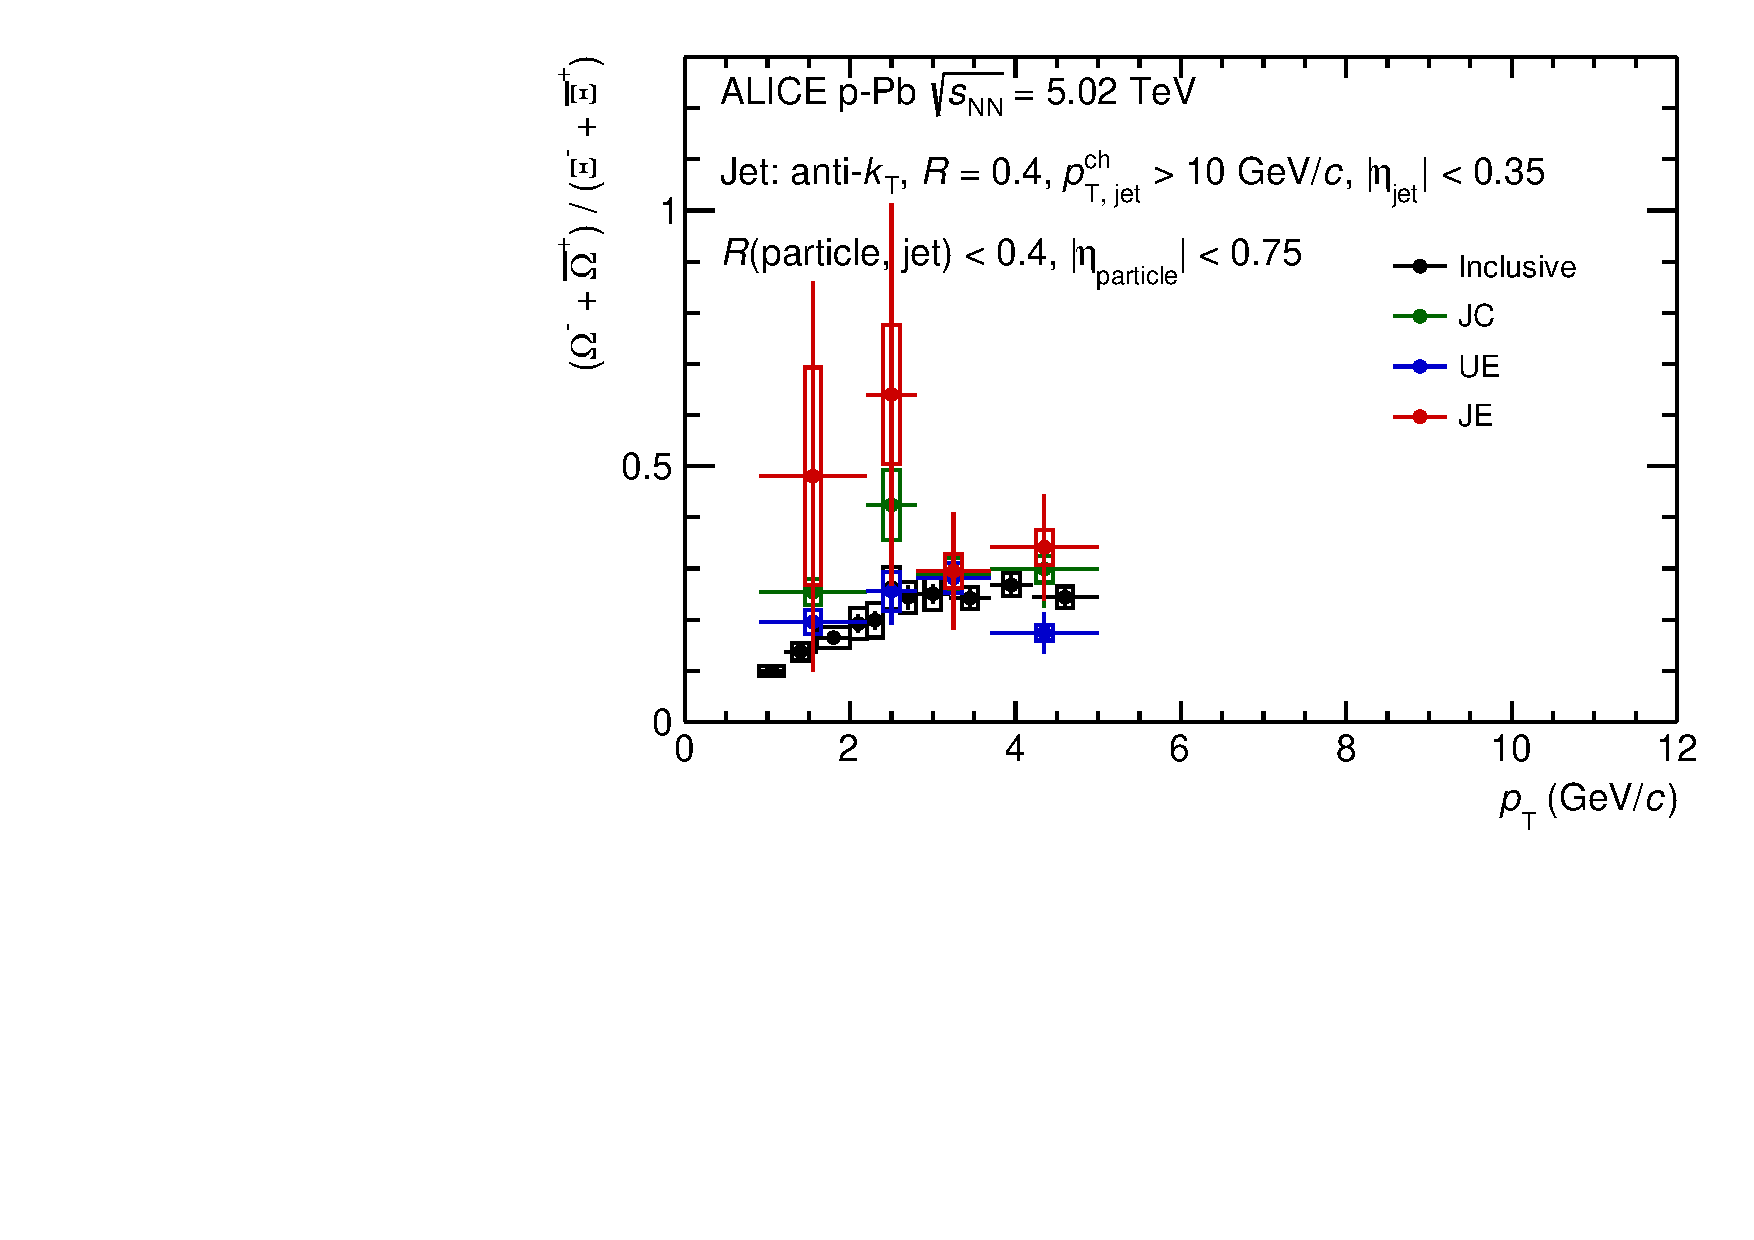
\includegraphics[width=.3\textwidth]{cf8_6}
	\end{center}
	\caption{Particle ratios.}
	\label{fig:pPbRatio}
\end{figure}

\subsection{Compare to models}
\label{subsec:ComToMod}
